\chapter{Characterising the beam} % (fold)
\label{prt:characterising_the_beam}
\section{Introduction} % (fold)
\label{cha:introduction}
Characterisation of the MuSIC beam was carried out over several years and through a number of experiments. Over the course of two years there were five runs making three significant measurements were made to characterise the beam: the total charged particle flux; the muon flux (by measuring the muon lifetime); and the muon momentum spectrum. The details of the runs are covered in table~\ref{tab:summary_music_beam_time} along with which experiments were carried out. Several other experiments were also carried out by other groups but these are not discussed here (i.e.\ neutron flux measurements, muonic x-ray measurements and Mo muon-bombardment experiment).
\begin{table}[htpb]
  \begin{center}
    \begin{tabular}{c|c|c}
      \multicolumn{2}{c|}{Dates}          & Measurements                                \\
      Start            & Stop             &                                             \\
      \hline                                                                             
      29 July 2010     & 31 July 2010     & Charged particle flux.                      \\
      \hline
      13 February 2011 & 16 February 2011 & Muon yield (lifetime).                      \\
      \hline
      \multirow{2}{*}{19 July 2011}
                       & \multirow{2}{*}{21 July 2011}
                                          & Muon yield (lifetime).                      \\
                       &                  & Muon yield (via muonic X-rays).             \\
      \hline
      22 October 2011  & 23 October 2011  & Neutron flux.                               \\
      \hline
      \multirow{3}{*}{18 June 2012}
                       & \multirow{3}{*}{22 June 2012}    
                                          & Muon momentum spectrum (via lifetime).      \\
                       &                  & Muon yield (via muonic X-rays).             \\
                       &                  & Mo muon-bombardment.                        \\
    \end{tabular}
  \end{center}
  \caption{A summary of the five MuSIC beam-times with notes on the measurements made.}
  \label{tab:summary_music_beam_time}
\end{table}

This chapter has been split into four sections: the rest of this section will cover be an introduction to the equipment used for the measurements, each of which will then be treated individually. Each measurement section will start by covering the set up, the results and analysis of the data.

The rest of this introduction will cover the equipment used to carry out each measurement as most of it was common to all the measurements.
\subsection{Scintillators Preparation} % (fold)
\label{sub:scintillator_preparation}
As discussed in section~\ref{sec:introduction_scintillation} scintillating materials produce light when charged particles travel through them. There are several categories of scintillator, those used for our measurements were plastic as they are easy to work with, inexpensive and available in a range of sizes. There are two main considerations in preparing a plastic scintillator: maximising light collection and preventing external light contamination. The standard approach to deal with both of these considerations is to polish and wrap the scintillator.

The scintillator surface is highly vulnerable to damage either through scratches or grease. Damage to the surface of the scintillator is problematic as it inhibits light collected through total internal reflection (TIR). Anything that reduces the amount of TIR increases the amount of light absorbed outside of the scintillator, where it cannot be detected. In order to prevent scratches, scintillators must be handled carefully and protective films are only removed at the last moment. As well as careful handling, the scintillators are cleaned to remove dirt and dust by polishing them with iso-propanol, this removes grease that can also degrade the surface.

Scintillators are generally wrapped with two thin layers: an inner reflective material and an outer blackout material. The inner layer is normally aluminium-mylar or foil, this is wrapped loosely in order to leave a small air gap that has been shown to increase the amount of TIR (and hence light collection)~\cite{air gap to increase light collection}. The outer layer is normally a black plastic wrap. This is carefully sealed with tape to prevent light leakage (another aid to this is obviously turning any lights off in the experimental area). An important consideration is to keep the layers as thin as possible in order to minimise energy deposition; to this end overlaps are kept to a minimum.

In order to attach sections of the scintillators together and to attach detectors to the scintillator optical cement and grease were used. Optical cement was used when a permanent fixing was required while grease was used if the components would need to be separated. To use the cement the components were cleaned using iso-propanol, then the two-part glue mixed and applied. A foam jig was used to hold the pieces in place whilst the cement set. When non-permanent joins were required, e.g.\ to attach MPPCs to WLS-fibres, optical grease was used to form the connection. Optical cement and grease have refractive indexes close to (if not the same as) that of the scintillators to maximise transmission either between sections of the scintillator (e.g.\ from the scintillator bulk to the WLS-fibre) or from the scintillator to the MPPC.
% Whilst a significant proportion of scintillator construction is dedicated to increasing reflection back into the scintillator, at the boundary to the MPPC it must be minimised to maximise the amount of light hitting the MPPC (rather than being reflected back into the scintillator).

% subsection scintillator_preparation (end)
\subsection{Multi-Photon Pixel Counters} % (fold)
\label{sub:multi_photon_pixel_counters}
Multi-Photon Pixel Counters (MPPCs, see figure~\ref{fig:images_intro_MPPC_from_hammamatsu_report}) are highly sensitive devices able to accurately count photons over a wide range of intensities. An MPPC is a small device (normally \( \mathcal{O}(1\times1) \)~mm\(^2\)) made from many Avalanche PhotoDiodes (APD) operated in `Geiger-mode'. Each individual APD is a single pixel within the MPPC. The APDs are connected together so that the MPPC's output is the sum of the outputs of the individual pixels. As can be seen in figure~\ref{fig:images_intro_hamamatsu_mppc_waveform_and_counts} there is clear banding that corresponds to the number of incident photons making an accurate obtainable as long as the system operates within the MPPC's limitations (discussed below).
\begin{figure}[hptb]
  \centering
    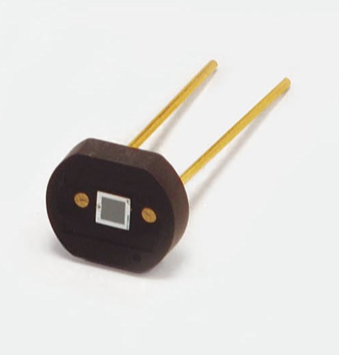
\includegraphics[width=.3\textwidth]{images/intro/MPPC_from_hammamatsu_report.png}
  \caption{Photograph of an MPPC (type S10362-11 with ceramic package) from the Hamamatsu technical report~\cite{hamamatsu_mppc_tech_report}}
  \label{fig:images_intro_MPPC_from_hammamatsu_report}
\end{figure}

\begin{figure}[hptb]
  \centering
    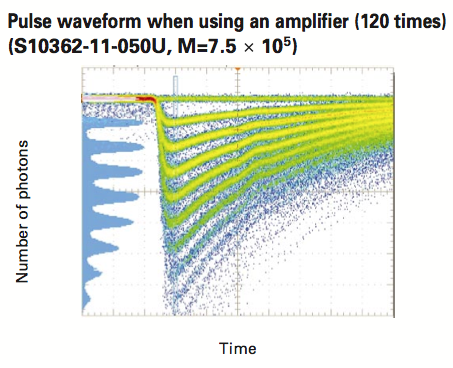
\includegraphics[width=.6\textwidth]{images/intro/hamamatsu_mppc_waveform_and_counts.png}
  \caption{Oscilloscope waveform for an MPPC with a histogram of peak voltage on the left. The histogram shows the clear discrimination between number of photons available on a MPPC. This type of MPPC has \(400\times50\times50 \mu\text{m}^2\) APDs in a \(1\times1\text{mm}^2\) package taken from~\cite{hamamatsu_mppc_tech_report}.}
  \label{fig:images_intro_hamamatsu_mppc_waveform_and_counts}
\end{figure}

APDs make use of the photoelectric effect and large voltages to produce an `avalanche' of electrons when triggered by an incident photon. A limitation to this system is that an individual APD's output is roughly constant regardless of the number of incident photons. Should the number of photons become comparable to the number of pixels then the MPPC becomes saturated and produces a constant signal as all the pixels fire, rather than clear bands as pixels fire in isolation. For the energy range predicted at MuSIC saturation is not considered to be a significant problem as the number of photons is predicted to be below the one hundred pixels used in our MPPCs (see figure~\ref{fig:sim_n_photons}). 

\begin{figure}[hptb] 
  \centering    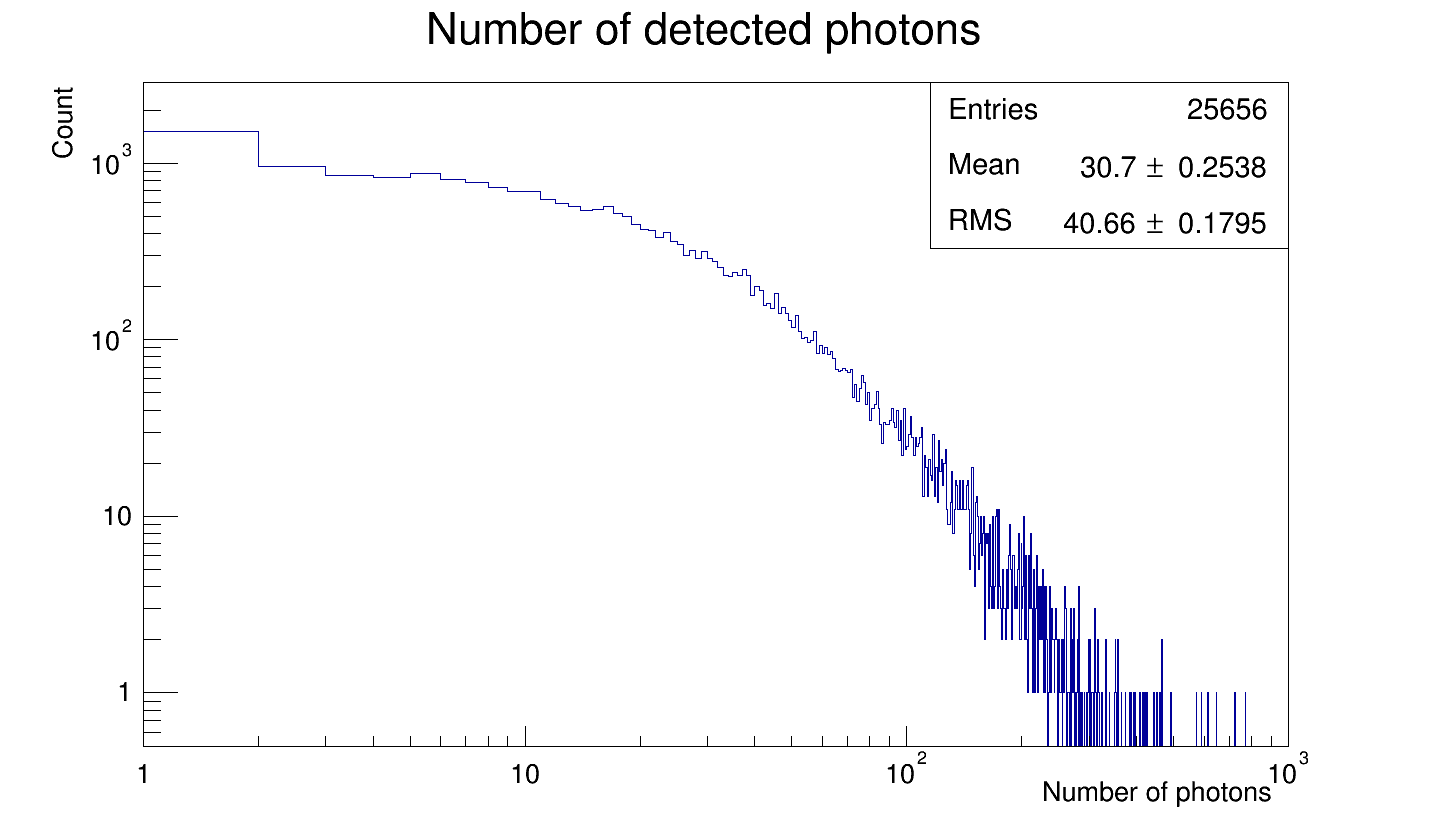
\includegraphics[width=.9\textwidth]{images/plot_generating_scripts/n_photons.png}
  \caption{Simulated distribution of number of photons reaching one of the MPPCs attached, via wavelength shifting fibre, to a \(380\times50\times3.5\)~mm\(^3\) scintillator.}
  \label{fig:sim_n_photons}
\end{figure}


An MPPC has several key attributes: Photon-Detection Efficiency (PDE), peak sensitivity, time resolution, operating voltage (\( V_0 \)), gain (\( M \)) and dark current. The PDE and peak sensitivity respectively describe the likelihood of detection of a photon of given wavelength (see figure~\ref{fig:images_intro_hamamatsu_pde_vs_wavelength}) and the wavelength that the MPPC is most sensitive to (typically \(\sim\)440~nm). Time resolution for MPPCs is generally very good, normally 200--300~ps for FWHM at the single photon level which is more than accurate enough for our purposes. The operating voltage is the potential required to make the MPPC work, due to variance in manufacture this is given individually for each MPPC and has to has to be set correctly for optimum performance, Hamamatsu's MPPCs have \( V_0 = 70\pm10 \)~V. The gain of the MPPC indicates the strength of the signal response to a photon, typical values are between \( 10^5 \) and \( 10^6 \), this corresponds to signals of \( \mathcal{O}(1\text{--}10) \)~\(\mu\)V which must be amplified for accurate measurement. The dark current is a measure of how noisy a particular MPPC is; it is the rate of false signals that have an effective strength equivalent to 0.5~photo-electron (p.e.). Typical values for the dark current are in the range 100--500 kcps (\(\times10^3\)~counts per second) these can be accounted for by correct setting of triggers.
\begin{figure}[hptb]
  \centering
    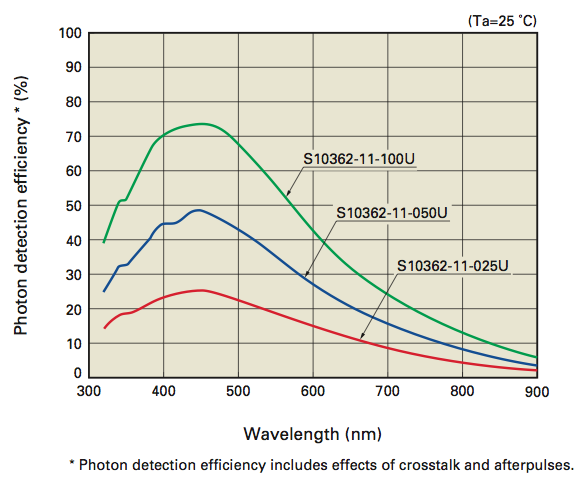
\includegraphics[width=.5\textwidth]{images/intro/hamamatsu_pde_vs_wavelength.png}
  \caption{MPPC Photon Detection Efficiency (PDE) as a function of photon wavelength. A range of pixel densities are shown (100, 400, 1600 pixels/\( 1\times1\text{mm}^2\) for the 100U, 050U and 025U models respectively) demonstrating the prime taken from~\cite{hamamatsu_mppc_tech_report}.}
  \label{fig:images_intro_hamamatsu_pde_vs_wavelength}
\end{figure}

As can be seen, whilst MPPCs have many useful features they do have several features that need careful treatment to make them useful: mainly amplification and noise reduction. These two problems are closely related and in fact, when treated properly one will often help with the other. Given the size of the signal from an MPPC it is obvious that amplification is required to make the signal useable, in fact, as will be discussed below, an unfiltered MPPC signal is too small for detection by most standard equipment. Amplification is done using linear amps which are applied as soon as possible to reduce noise due to cabling as well as attenuation. 
% As well as amplification simple filters are applied to the bias voltage and signal to help reduce noise (see figure~\ref{CIRCUIT DIAGRAM}). Careful ground was also required to reduce noise, this was mainly carried out by ensuring shared ground between different modules.

% subsection multi_photon_pixel_counters (end)
\subsection{Secondary Emission Chamber} % (fold)
\label{sub:secondary_emission_chamber}
As well as studying the resultant beam, knowledge of the initial proton beam is essential for normalisation. This is done using a Secondary Emission Chamber (SEC). A SEC uses thin foils of gold placed within a strong electrical potential. When protons pass through the foils a small number of electrons are produced as part of ionisation, these can then be collected and counted. The SEC only measures a fraction of the beam and even then, only indirectly. In order to calibrate the SEC runs are performed in which the entire proton beam is absorbed with a copper block downstream of the SEC. Measurement of the total current produced by the block can then be used to determine the fraction absorbed by the SEC, and hence the conversion factor. Measurement of the SEC was carried out using scalers (see below) that counted the cumulative charge passing through the SEC.

% subsection secondary_emission_chamber (end)

\subsection{NIM, CAMAC and VME} % (fold)
\label{sub:nim_and_camac}
Rather than develop custom data acquisition hardware, a modular crate system was used. A crate system supplies power and mechanical fixings for a range of modules, these modules can then be connected together to produce a system. Three crate systems were used: Nuclear Instrument Module (NIM), Computer Automated Measurement And Control (CAMAC) and Versa Module Eurocard bus (VMEbus or VME). NIM supplies power only, whilst CAMAC and VME provide a `backplane' through which data can be transferred to a control card.

NIM modules were primarily used to provide signal processing and data acquisition logic. The CAMAC and VME crates were used for data readout. Ultimate control and storage was carried out using a PC which recorded the data for later analysis. The rest of this section will discuss the basic modules used in NIM, CAMAC and VME.
\subsection{Discriminators} % (fold)
\label{ssub:discriminators}
A discriminator works by producing a digital signal when an analogue input-signal exceeds some preset threshold. Converting the analogue signal to digital makes it much easier to manipulate as many other modules can only use a digital signal. The discriminators were powered by NIM modules and had their thresholds set manually.

Discriminators were used to signal when a certain number of photons were detected by an MPPC i.e.\ when a particle had passed through the scintillator. As the discriminators have a minimum threshold of \(\sim\)25~mV the MPPC signals were amplified to make them useable. As every MPPC has a different gain the thresholds for the discriminators had to be set individually. To normalise between MPPCs the discriminator thresholds were set based on the number of photons the analogue signal corresponded to (see figure~\ref{fig:images_intro_hamamatsu_mppc_waveform_and_counts}). The trigger level (in p.e.)\ was the same for all MPPCs and was chosen to maximise the signal to noise ratio, a typical value was \(\sim2.5\)~p.e. which suppressed most of the dark current without compromising sensitivity to charged particles. An oscilloscope could then used to translate the photon (p.e.)\ threshold into a voltage threshold (in mV) that can be used by the discriminator.

% The thresholds had a standard minimum value of \(\sim\)25~mV, in order to meet this linear amplifiers were used to boost the MPPC signal enough to be detectable. 

% subsubsection discriminators (end)
\subsection{Gates and Latches} % (fold)
\label{ssub:gates}
Gates are a set of modules that generally have several related functions. Depending on the mode they can change the length of a signal, delay it, `latch' it or start a clock signal. The first two modes are generally used for creating `gates' (on or off signals) for other modules: e.g.\ turning on a module to record the shape of a signal or indicating to the PC that their is data waiting to be read. A `latch' is a signal that remains on until another signal switches it off, these are often used when it's unclear how long something will take e.g.\ sending data to the PC. Clock signals were generally used as calibration information for other measurements e.g.\ recording the SEC.

% Gates are modules that, when triggered produce an altered signal compared to the input. As well as delaying and lengthening signals gates can also be used in `latch' (or flip-flop) mode. Gates only accept digital signals but can create delays of up to 1~s, and equally change the length by similar amounts. In latch mode the input signal starts the output whilst another input resets it. Latch mode is used to create busy signals by using the input to indicate when the DAQ is processing an event and a signal from the PC to reset it.

% subsubsection gates (end)
\subsection{Logic units} % (fold)
\label{ssub:logic_units}
Logic units provide boolean logic (`AND', `OR', `NOT') for processing digital signals. The limiting factor is the number of inputs that can be combined and the complexity of the combinations. Normally signals are combined in a block with a single module having several discrete blocks. Each block will perform a single logical operation (OR or AND) on its inputs. The inputs of a block can either be normal or negated. A block (or sometimes the entire module) will generally have a veto signal that will stop outputs until the veto is cleared.

Logic units were generally used for simple tests such as checking that all MPPCs on a scintillator had triggered, this helped reduce the number of false positives in addition to the application of a discriminator. Logic units were also used to prevent attempts process to events at once: if a second event arrived before the previous event was fully processed then the second event was ignored. This leads to `dead time' but is unavoidable.

% subsubsection logic_units (end)
\subsection{Scaler} % (fold)
\label{ssub:scaler}
A scaler is a counting module. It receives a digital input, that when asserted, increments its counter. The most important factor of a scaler is its maximum speed (the maximum input frequency). Events that occur more rapidly than the input frequency will not be properly counted (either not being counted at all or counted as a single event), a typical maximum input frequency is 100~MHz. Most scalers can be daisy-chained together in case their maximum value is exceeded and some allow multiple inputs that can be counted independently. NIM scalers will generally some form of direct readout (e.g.\ a display) whilst VME/CAMAC modules will be readout via their data-bus. 

% One of the simplest forms of read out is a count of triggers, this is what a scaler does. The primary concern with a scaler is the input specification to trigger a count as well as the maximum speed at which the unit can count. Modules can either be used with NIM, CAMAC or VME. When the rate is high or the maximum count is low multiple scalers can be daisy-chained together to provide carry over. 
z
% subsubsection scaler (end)
\subsection{Analogue to Digital Converter} % (fold)
\label{ssub:analogue_to_digital_converter}
There are two primary attributes of an MPPC signal that were measured: its size and its separation from other signals. In order to measure the size of the MPPC signal an Analogue to Digital Converter (ADC) was used. ADCs work in a variety of ways depending on the exact type of measurement they are making, two common versions used at MuSIC were Peak Sensing ADC (PS-ADC) and Charge-integrating ADCs (QDC). Both types of ADC measure a component of the input analogue signal, the PS type measures the peak voltage whilst the CI measures the integrated charge, both make these measurements only when enabled by the ADC's `gate'. The ADC's gate is normally set to be slightly longer than the expected signal from an MPPC, i.e.\ \( \sim \)50~ns. 

Several factors define the ADC: the number of bits it is able to read out, the range of input signals that it can measure, its linearity, digitisation/read time (`dead time') and number of channels. The number of bits the ADC has, the range and its linearity work together to determine the accuracy of the ADC; the number of bits determines the resolution between any two values, the range determines the the values that the ADC can measure whilst the linearity maps measured values to actual voltages. Dead time measures how long is required to measure the analogue signal and how long it takes to then send the digitised values to the controlling PC i.e.\ for how long the module is inoperative, `dead'. The number of channels on an ADC is a measure of how many inputs it can measure simultaneously, normally one is ascribed to each MPPC so that the triggering signal can be recorded.

A key feature of using an ADC is the pedestal, obviously any analogue signal is going to have some noise that represents its zero level, in an ADC this manifests as a large peak in the lower bins of the ADC, removal of the pedestal is often done by the ADC itself and through DAQ but it does sometimes have to be removed from the data as well.

% subsubsection analogue_to_digital_converter (end)
\subsection{Time to Digital Converter} % (fold)
\label{ssub:time_to_digital_converter}
A Time to Digital Converter (TDC) measures the time difference between two (or more) signals. Similarly to the ADC the core parameters for a TDC are the number of bits, the TDC's range, its linearity, its dead time and number of channels. A TDC normally takes a single `start' signal and will then measure the delay(s) been that first signal and any further signals on the other channels (`stops'). A useful variant on the TDC used in later experiments was the Multi-Hit TDC (MH-TDC). Rather than measure a single start/stop pair for each channel the MH-TDC uses a buffer to record every incoming event, when the `start' signal is received it signals that the current state of the buffer (and some trailing amount) should be recorded. Using this method, events proceeding the start signal can be recorded as well as those afterwards.

% subsubsection time_to_digital_converter (end)
\subsection{Registers} % (fold)
\label{ssub:registers}
Registers are similar to the gate modules discussed above except that they are either or written directly by the PC. Registers are two key uses in our systems: either indicating (an `interrupt') to the controlling PC that their is data to be read or to reset the DAQ after a successful read. Interrupts were formed using a logic unit and a gate: once a trigger had be formed by the logic unit the gate would delay the interrupt signal long enough for the ADC & TDC digitisation to complete then signal the controlling PC. The PC's reset signal was used to unlatch the veto signals that prevented doubling up of data as well as clear any other latches used by the system.

% Control registers are fairly simple devices but very useful in general control, they act as a simple toggle that can either send or receive a signal to the controlling PC. The main use of registers is to form an interrupt; used this way once data has been taken the ready state of the system can be signalled to the PC and the PC can begin read-out. The interrupt is often delayed so that full digitisation can occur although has to be carefully gauged to prevent excessive dead time. The second common use is to reset the system once read-out has completed, this normally means resetting a latched gate that has been holding the system in veto.

% subsubsection registers (end)
% subsection nim_and_camac (end)
% section experimental_technique (end)
% chapter introduction (end)
\section{Charged Particle flux} % (fold)
\label{cha:charged_particle_flux}
% TODO Pictures of set ups
% TODO Diagrams of set ups
The first experiments carried out at MuSIC aimed to establish the barest understanding of the beam, the flux of charged particles. Whilst this experiment yielded useful data it was ultimately a prototype for the technology and a way to test and develop the techniques for later experiments.

Two measurements of the charged particle flux were made: one using a long strip scintillator that measured the flux at a range of heights and a second that used a smaller disk that measured the flux at a number of points across the face of the disc. These measurements were made during two different beam-times but will be discussed together as they have a lot of their designs in common.

These early experiments had DAQ designs that were ultimately superfluous as the data it yielded was not used; this design is included for completeness.
\subsection{Experimental Set Up} % (fold)
\label{sec:experimental_set_up}
The experimental design for both measurements was broadly the same: the scintillators both had four MPPCs attached, NIM was used logic for basic triggering whilst read-out was performed via CAMAC crates, data was recorded on a PC and analysed afterwards. The scintillators were both wrapped with aluminium foil and black wrap and the MPPCs attached via optical cement (see table~\ref{tab:charged_particle_flux_scint_details}).
\begin{table}
  \begin{center}
    \begin{tabular}{c|c|c|c}
      Shape  &  Volume (mm\(^3\))            &  MPPCs  &  MPPC positions                    \\
      \hline
      Strip  &  \(380 \times30\times10\)     &  4      &  \( \pm 5 \)~mm on each ends.      \\
      Disk   &  \( 35^2\times\pi\times20\)  &  4      &  Radially, every 90\( ^{\circ} \). \\
        
    \end{tabular}
  \end{center}
  \caption{Details of the scintillators used for the two measurements of the charged particle flux.}
  \label{tab:charged_particle_flux_scint_details}
\end{table}

The aim of these early experiments was to make three measurements: the total trigger rate, the difference in arrival times of light at the MPPCs and the distribution of the number of firing pixels at each MPPC. The total trigger is proportional to the flux of charged particles through the scintillator. It was hoped that the timing difference between MPPC firings could be correlated to the position of the interaction within the scintillator (this was ultimately incorrect). The distribution of the number of firing pixels was hoped to give some idea of the energy deposited, and possible the types of particles. 

Ultimately only the measurement of the trigger rate was successful. The trigger rate is proportional to the charged particle flux as long a the dead time is essentially nil. To ensure this, as discussed below, a simplified DAQ system was used and MuSIC was run with a reduced beam current (\(<1\)~nA instead of the MuSIC design current of \(~1\)~\(\mu\)A). Another concern for measuring the charged particle flux is minimally ionising particles, by definition these particles will scintillate the least making their detection difficult, to mitigate this a thicker scintillator (20~mm) was used for the second measurement in which more energy would be deposited.

The trigger rate DAQ system was a subset of the full DAQ used to measure the time and energy:
\begin{enumerate}
  \item Amplify the MPPC signal to a detectable level (see section~\ref{sub:multi_photon_pixel_counters}).
  \item Use a discriminator to remove noise.
  \item Use an AND module to form a trigger and raise a veto based on the coincidence of events from all MPPCs.
  \item Record the analogue MPPC signal using an ADC.
  \item Use the trigger to start the TDC.
  \item Delay three of the remaining signals by an amount to form the stops to the TDC.
  \item Remove the veto on the system once read out is complete.
\end{enumerate}
This can be seen as a schematic in figure~\ref{fig:MuSIC1_DAQ_Block}. 

\begin{figure}[hptb]
  \centering
  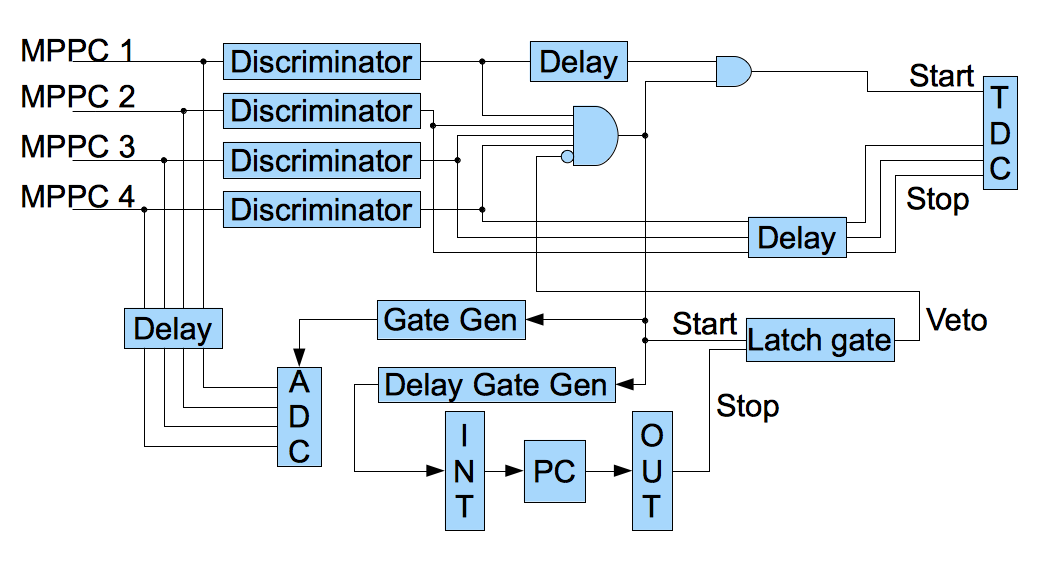
\includegraphics[width=.9\textwidth]{images/charged_flux/MuSIC1_DAQ_Block.png}
  \caption{Schematic of the DAQ used for measuring the charged particle flux. Horizontal blocks indicate NIM units whilst vertical units were mounted in a CAMAC crate. The two `AND' blocks were made using NIM modules.}
  \label{fig:MuSIC1_DAQ_Block}
\end{figure}

To make the final measurement of the trigger rate, the majority of the DAQ was ignored and the four-fold coincidence counted using a scaler. By counting the raw triggers, affects of dead time could be negated and a truer value for the number of interactions obtained. For the 1D experiment measurements were made over 50~s with control done via hand, this obviously had limitations 

The positions of the two experiments are given in table~\ref{tab:flux_setup} with respect to the centre of the beam-pipe. `By-eye' readout of the 1D measurement was done using a display mounted on the scaler used to count triggers. For the 2D measurement a CAMAC module was used that was read out by computer.
\begin{table}
  \begin{center}
    \begin{tabular}{c|c|c|c|c|c}
      Measurement  &  \multicolumn{3}{c|}{Distance from centre of beam (cm)}         &  Scaler    &  Readout \\
      &    Horizontal    &       Vertical              &  Longitudinal  &  Time (s)  &          \\
      \hline            
      1D           &  0               &  \(-5\), \(-15\), 0, 15, 5  &       6        &  50        & By-eye   \\
      2D           &  \(-17\), 0, 17  &  \(-16\), 0, 20, 25         &       85       &  20        & CAMAC    \\
    \end{tabular}
  \end{center}
  \caption{Positions at which the charged particle flux was measured, 1D refers to the first run in which only the vertical displacement was measured, 2D refers to the second run in which horizontal measurements were also take. The distances from the beam-pipe were 6~cm for 1D measurements and 85~cm for 2D, this was due to mechanical constraints.}
  \label{tab:flux_setup}
\end{table}

% section experimental_set_up (end) 
\subsection{Detector efficiency} % (fold)
\label{sec:detector_efficiency}
As well as making measurements of the charged particle flux another important measurement, made soon after the second beam time, was measurement of the efficiency of the circular detector. This was done using 3 large Photo-Multiplier Tubes (PMT) attached to large (\( 40\times40\times1 \)~cm\(^3\)) scintillator paddles. Measurement of the disk detector was calculated using the ratio of detections by the PMTs to detection by the MPPCs (once size considerations had been taken into account).

The test procedure for this measurement was to do long runs with the PMT paddles sandwiching the disk then compare the number of cosmic rays detected in the paddles compared to those detected by the disk. First all remaining MPPCs were tested (one had become irrevocably damaged during beam time) then pairs were tested. Testing consisted of counting the occurrence of three-fold coincidence on the PMTs and either two or three fold coincidence on the MPPCs. Data was taken for approximately one day for each configuration. The results of this measurement are shown in table~\ref{tab:music2_eff}.

\begin{table}
  \begin{center}
    \begin{tabular}{c | c | c | c | c | r@{~\( \pm \)~}l}
      \multirow{2}{*}{Configuration} 
                     &  Run Time             &  MPPC   &  PMT        &  \multirow{2}{*}{Efficiency} 
                                                                                    &  \multicolumn{2}{c}{Adjusted}   \\
                     &  (\(\times 10^3\)~s)  &  Count  &  Count      &              &  \multicolumn{2}{c}{Efficiency} \\
      \hline
      123            &  86.0                 &  1651   &  1,161,165  &  0.00142     &  0.0591 & 0.0015  \\
      12             &  92.3                 &  6055   &  1,229,389  &  0.00493     &  0.2048 & 0.0026  \\
      13             &  87.1                 &  5653   &  1,179,116  &  0.00479     &  0.1993 & 0.0027  \\
      23             &  84.4                 &  3999   &  1,129,137  &  0.00354     &  0.1472 & 0.0023  \\
        
    \end{tabular}
  \end{center}
  \caption{Summary of the data taken for measuring the MPPC detector efficiency. Configuration refers to which of the three MPPCs were tested. The efficiency is the simple ratio of the MPPC count to the PMT count whilst the adjusted efficiency has been scaled by the ratio of the areas of the scintillators, i.e.\ by \( \frac{40\times40}{\pi3.5^2} \).}
  \label{tab:music2_eff}
\end{table}

Assuming that the total efficiency (\( \epsilon_t \)) is the product of the individual efficiencies (\( \epsilon_{1,2,3} \)) then the it can be expressed as:
\begin{align}
  \epsilon_t &= \epsilon_1  \epsilon_2  \epsilon_3
\end{align}
With the measured efficiencies of the pairs of MPPCs we can calculate the individual efficiencies by solving:
\begin{align*}
  \epsilon_{12} &= \epsilon_{1} \epsilon_{2} &\implies   \epsilon_{1}  &= \frac{\epsilon_{12}}{\epsilon_{2}}                       \\
  \epsilon_{13} &= \epsilon_{1} \epsilon_{3} &\implies   \epsilon_{2}  &= \frac{\epsilon_{12}\epsilon_{3}}{\epsilon_{13}}          \\
  \epsilon_{23} &= \epsilon_{2} \epsilon_{3} &\implies   \epsilon_{3}  &= \sqrt{\frac{\epsilon_{23}\epsilon_{13}}{\epsilon_{12}}}  \\
\end{align*} 
This can be generalised to:
\begin{align*}
  \epsilon_{i} &= \sqrt{\frac{\epsilon_{ij}\epsilon_{ik}}{\epsilon_{jk}}} \label{equ:individual_eff}
\end{align*}
Where \( \epsilon_i \) is a single efficiency we want to calculate and \( \epsilon_{jk} \) is the combined measurement of the other two efficiencies. Applying this to table~\ref{tab:music2_eff} we get the efficiencies for the MPPCs shown in table~\ref{tab:calculated_individual_eff}. It's important to note that these efficiencies represent more than just the individual MPPC's quantum efficiency but the entire gestalt of systematic effects that contribute to the efficiency of the specific MPPC including scintillator acceptance (both geometric and energetic), light collection and transmission. As can be seen the estimated total efficiency ends up being larger than what was actually measured but this is to be expected as the system assumes all the efficiencies are completely independent of one another. Using these values the average efficiency of a single MPPC can be calculated and given an error as seen in the final line of the table.

\begin{table}
  \lineup
  \begin{center}
    \begin{tabular}{c|r@{~\(\pm\)~}l}
      MPPC  &  \multicolumn{2}{c}{Efficiency} \\
      \hline
      1  &  0.5265 & 0.0064  \\
      3  &  0.3786 & 0.0046  \\
      2  &  0.3889 & 0.0048  \\
      \hline
      \( 123_{Calc} \)  &  0.0775  &  0.0016  \\
      \( 123_{Meas} \)  &  0.0591  &  0.0015  \\
      \hline 
      \( \epsilon_{\text{MPPC}} \)  &  0.431\0 & 0.067 \\
         
    \end{tabular}
  \end{center}
  \caption{Efficiencies of individual MPPCs calculated using the values from table~\ref{tab:music2_eff}, and equation~\eqref{equ:individual_eff}. The two values below the line represent the total efficiency as calculated using the individual values and the measured value. Note: these values also include any acceptance effects and the light collection efficiencies of the scintillator.}
  \label{tab:calculated_individual_eff}
\end{table}


% section detector_efficiency (end)
\subsection{Results} % (fold)
\label{sec:results}

Prior to the main experiments the conversion factors from SEC count to proton current was determined, these values were determined to be, respectively for the 1D and 2D measurement: 0.03408~nA and 0.01514~nA . The results from the measurements are presented in table~\ref{tab:1d_res}, for the 1D case, and table~\ref{tab:2d_res} in the 2D case. The counts were converted to rates and the flux calculated using:
\begin{align}
  j &= \frac{F(C - C_{off})}{I_{p}} \\
  I_{p} &= K(S - S_{off})
\end{align}
where \(j\) is the flux, \(F\) is a scaling factor, \(C\) is the trigger count with the beam on, \(C_{off}\) is the background trigger rate (i.e.\ with the beam off), \( I_{p} \) is the proton current, \(S\) is the SEC count, \(S_{off}\) is the SEC count with the beam off and \(K\) is the SEC to current conversion factor. The scaling factor, \(F\), was  used in normalise runs with different conditions. For the 1D measurement there was a discrepancy between the first four and last five measurements due to damage to the MPPCs (one broke and another became detached from the scintillator). The 2D measurements were made at a larger distance than the 1D measurements as there was another experiment upstream that prevented closer positioning. The upstream experiment was making the muon lifetime measurement discussed below, it consisted of two scintillators on either side of stopping target. The stopping target was initially 5~mm of copper  that was changed to 20~mm of magnesium for the final 3 runs.

% During the 2D measurements some of the runs were made with an upstream experiment in a different configuration; a stopping target of 5~mm of copper to 20~mm was used initially and changed to to magnesium for the last 3 runs.
\begin{table}
  \begin{center}
    \begin{tabular}{ r | r | c | c | c | c | r@{~\(\pm\)~}r } 
      Height  &  \multicolumn{2}{c|}{Trigger Count} &  \multicolumn{2}{c|}{SEC Count}  &  Factor  &  \multicolumn{2}{c}{Flux}          \\
      (cm)    &        Beam on  &  Beam off         &  Beam on &  Beam off             &          &  \multicolumn{2}{c}{(nA\(^{-1}\))} \\
      \hline
        0      &  2,151,736  &    \multirow{4}{*}{30}   &   1,255  &  \multirow{4}{*}{381} &  \multirow{4}{*}{\( 1.0\pm0.0 \)}  
                                                                                                  &  72,200  & 3,600 \\
      \(-5 \)  &  1,438,685  &                          &   1,286  &                       &          &  47,000  & 2,300 \\
      \(-15\)  &    446,302  &                          &   1,212  &                       &          &  15,800  &   810 \\
      \(-15\)  &    502,596  &                          &   1,208  &                       &          &  17,800  &   920 \\
      \hline            
        5      &  1,663,702  &   \multirow{4}{*}{83}    &   1,298  &  \multirow{4}{*}{398} &  \multirow{4}{*}{\( 1.646\pm0.023 \)}  
                                                                                                  &  89,300 & 4,600  \\
        5      &  1,420,836  &                          &   1,142  &                       &          &  92,200 & 5,300  \\
       15      &  1,080,170  &                          &   1,336  &                       &          &  55,600 & 2,800  \\
       15      &  1,185,051  &                          &   1,371  &                       &          &  58,800 & 2,900  \\    
       \hline
        0      &  1,307,015  &         34               &   1,298  &             404       & \(1.646\pm0.023\)
                                                                                                  &  70,600 & 3,600  \\
    \end{tabular}
  \end{center}
  \caption{Summary of the results from the measurement of the vertical charged particle flux. The errors on the counts are the square root of the value. Counts were taken for \( 50\pm0.5 \)~s, the errors on both count and time are included in the final flux calculation. The factor was taken to be the ratio of two measurements made at 0~cm. The 0~cm measurements were used as this was the only pair of measurements that were made with the experiment in both conditions (i.e.\ all MPPCs functional and later, with one broken and another damaged). The error on the factor is the errors on the two 0~cm values added in quadrature.}
  \label{tab:1d_res}
\end{table}

\begin{figure}[hptb]
  \centering
  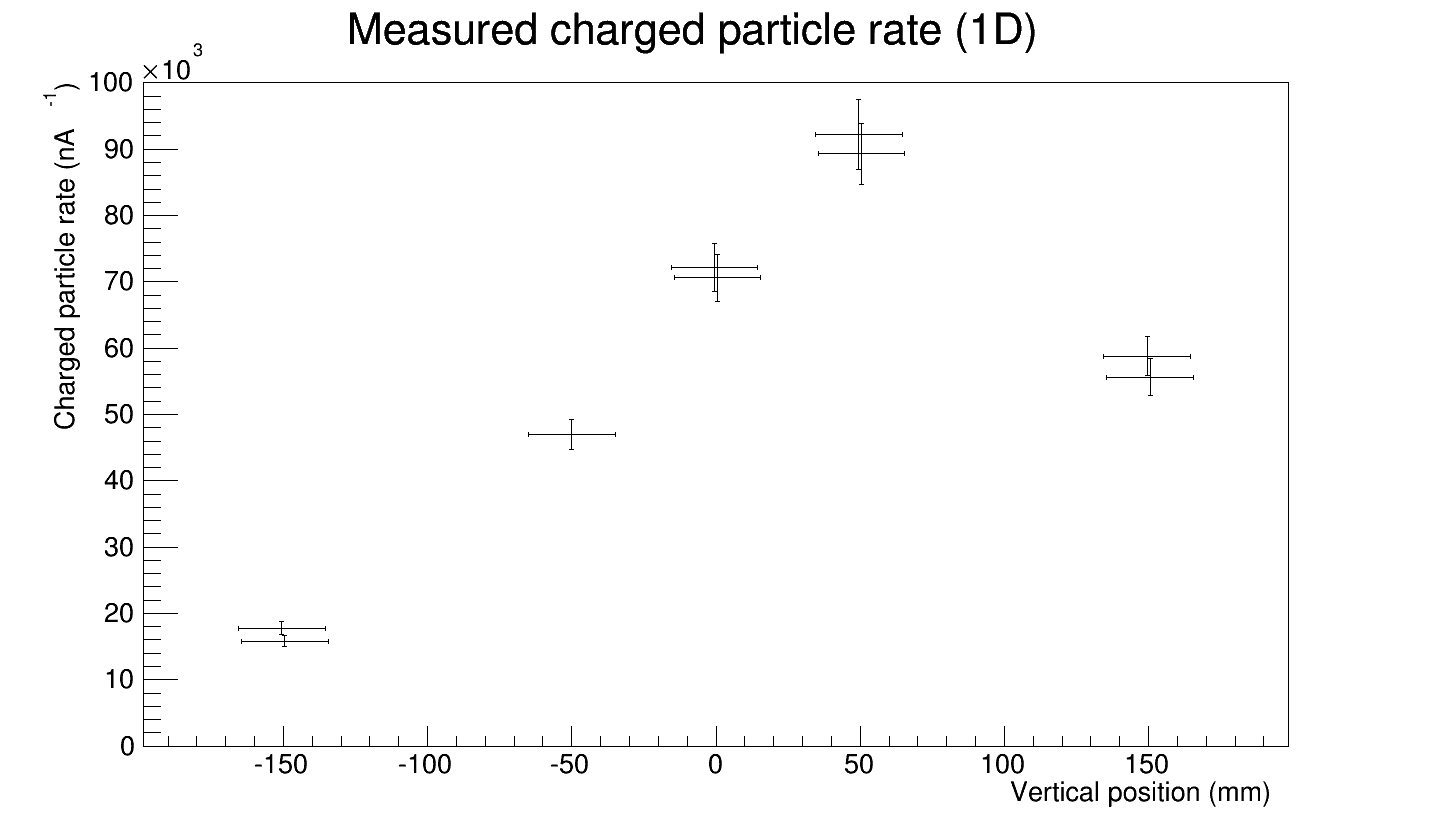
\includegraphics[width=.9\textwidth]{images/plot_generating_scripts/measured_1d_charged_flux.png}
  \caption{Measurement of the 1D charged particle flux as given in table~\ref{tab:1d_res}. Where two measurements were made at a single location an offset has been applied to the point to allow clearer reading of the plot, the measurements were actually at the same position. The errors on the vertical position are the width of the scintillator used.}
  \label{fig:images_hit_rate_rescaled}
\end{figure}

\begin{table}
  \begin{center}
    \begin{tabular}{r|r|r|c|c|c|r@{~\(\pm\)~}r}
      \multicolumn{1}{c|}{X}     &   \multicolumn{1}{c|}{Y}    &  \multicolumn{2}{c|}{Trigger Count}  &  \multicolumn{1}{c|}{SEC Count}  &  \multicolumn{1}{c|}{Factor}  &  \multicolumn{2}{c}{Flux}     \\
      \multicolumn{1}{c|}{(cm)}  &  \multicolumn{1}{c|}{(cm)}  &         \multicolumn{1}{c|}{Beam On}  &  \multicolumn{1}{c|}{Beam Off}         &  \multicolumn{1}{c|}{Beam On}    &          &  \multicolumn{2}{c}{(nA\(^{-1}\))}   \\
      \hline
        0      &    0      &           68,761 & 58                &   51        &  \multirow{2}{*}{\(1.0\pm0.0\)}
                                                                                           &   5,400  &  1,000 \\
      \(-17\)  &   20      &          117,947 & 58                &   51        &          &   9,300  &  1,700 \\
      \hline
      \(-17\)  &  \(-16\)  &           39,528 & 48                &   68        & \multirow{8}{*}{\(1.0\pm0.0\)}  
                                                                                           &   2,200  &    330 \\
      \(-17\)  &    0      &           97,190 & 78                &   73        &          &   5,010  &    710 \\
       17      &    0      &           63,160 & 91                &   76        &          &   3,110  &    430 \\
       17      &   20      &          105,097 & 88                &   71        &          &   5,590  &    810 \\
       17      &  \(-16\)  &           27,010 & 55                &   67        &          &   1,540  &    230 \\
        0      &  \(-16\)  &           43,634 & 97                &   69        &          &   2,400  &    350 \\
        0      &   20      &          142,536 & 73                &   64        &          &   8,600  &  1,300 \\
        0      &    0      &           75,376 & 60                &   66        &          &   4,360  &    660 \\
      \hline
         0      &   25     &           45,950 & 35                &   46        &   \multirow{3}{*}{\(1.784\pm0.008\)}
                                                                                           &   7,300  &  1,500 \\
       \(-17\)  &   25     &           69,582 & 119               &   47        &          &  10,800  &  2,100 \\
         0      &   20     &           80,088 & 238               &   60        &          &   9,200  &  1,500 \\
    \end{tabular}
  \end{center}
  \caption{Table of the results from the 2D measurement. All measurements were made over \( 20\pm0.001 \)~s apart from the first two measurements of the trigger count with the beam off which were made over \( 11\pm0.001 \)~s. Counts were made using a CAMAC controlled scaler and an enable gate triggered via interrupt register. The column for `SEC, beam off' is elided as it was constant at 9. The errors on the counts are the square root of the value, errors on the time are also propagated through the calculation.}
  \label{tab:2d_res}
\end{table}
 
\begin{figure}[hptb]
  \centering
  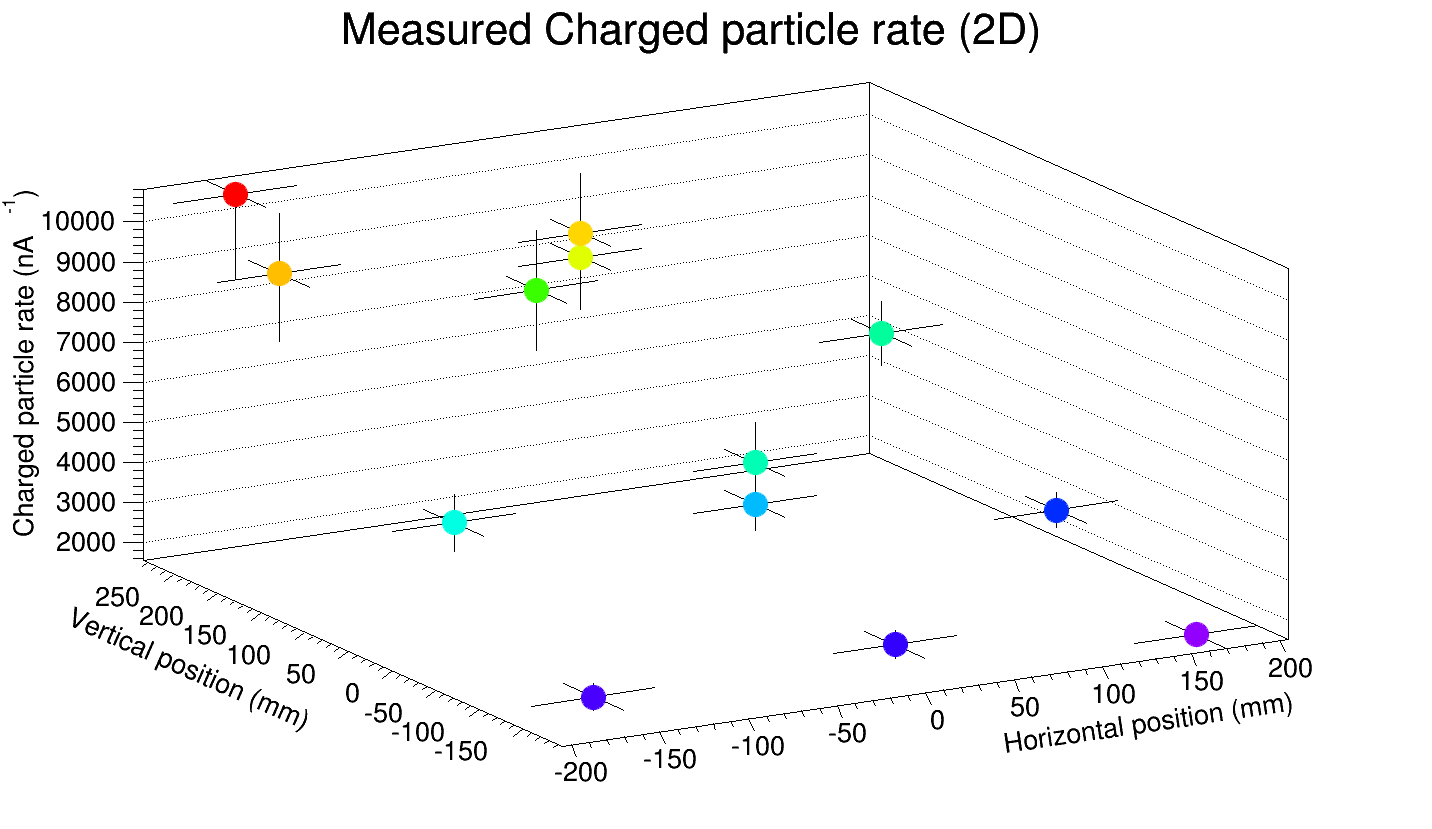
\includegraphics[width=.9\textwidth]{images/plot_generating_scripts/measured_2d_charged_flux.png}
  \caption{2D plot of the charged particle flux across the front of the MuSIC beam pipe. The final three measurements were rescaled using the ratio of the two measurements at \((0,20)\)~cm.}
  \label{fig:2D_flux}
\end{figure}
 
% section results (end)
\subsection{Analysis} % (fold)
\label{sec:analysis}
As can be seen from the figures~\ref{fig:images_hit_rate_rescaled}~and~\ref{fig:2D_flux} the beam spot is positioned slightly up and to the left of the centre of the pipe. As figure~\ref{fig:sim_2d_charged_particle_flux} shows both measurements agree on the general position of the beam spot. The measurements are not directly comparable due to the differences in both scintillator volume and position with respect to the end of the beam-pipe. Obviously the flux for the 2D measurement is generally lower due to smaller scintillator and greater distance from the beam-pipe.

The detector efficiency measurement for the 2D apparatus allows a more accurate calculation of the flux whilst also providing a bench-mark efficiency for future uses of the scintillator/MPPC configuration. 

The biggest problem, and one which was a cause of many problems, was the fragility of the MPPCs. Both the MPPC itself and the optical cement that bonded them to the scintillator were liable to break and this caused many problems that could not be easily fixed. 

A signifiant issue with the 1D measurement is the lack of a confirmation measurement that allows verification of the scaling but even if the re-scaled points are ignored then they confirm that the beam spot is in the upper half of the pipe, a measurement later confirmed by the 2D measurement. 

Comparing the measured and simulated rates yields some interesting features. There is broad agreement on the general shape of the distribution but, using normalised plots, it appears that the measured charged particle rate for the 1D measurement is consistently higher than the simulated value by a factor of between 2 and 10. No obvious explanation of this presents itself as the measured value, should be, a lower bound whilst the simulated value should be closer to the `true' value due to lack of detector affects and similar. Whilst this suggests that further development of the G4BL simulation is required it is encouraging that MuSIC is performing above expectations.

% \begin{figure}[hptb] 
%   \centering
%     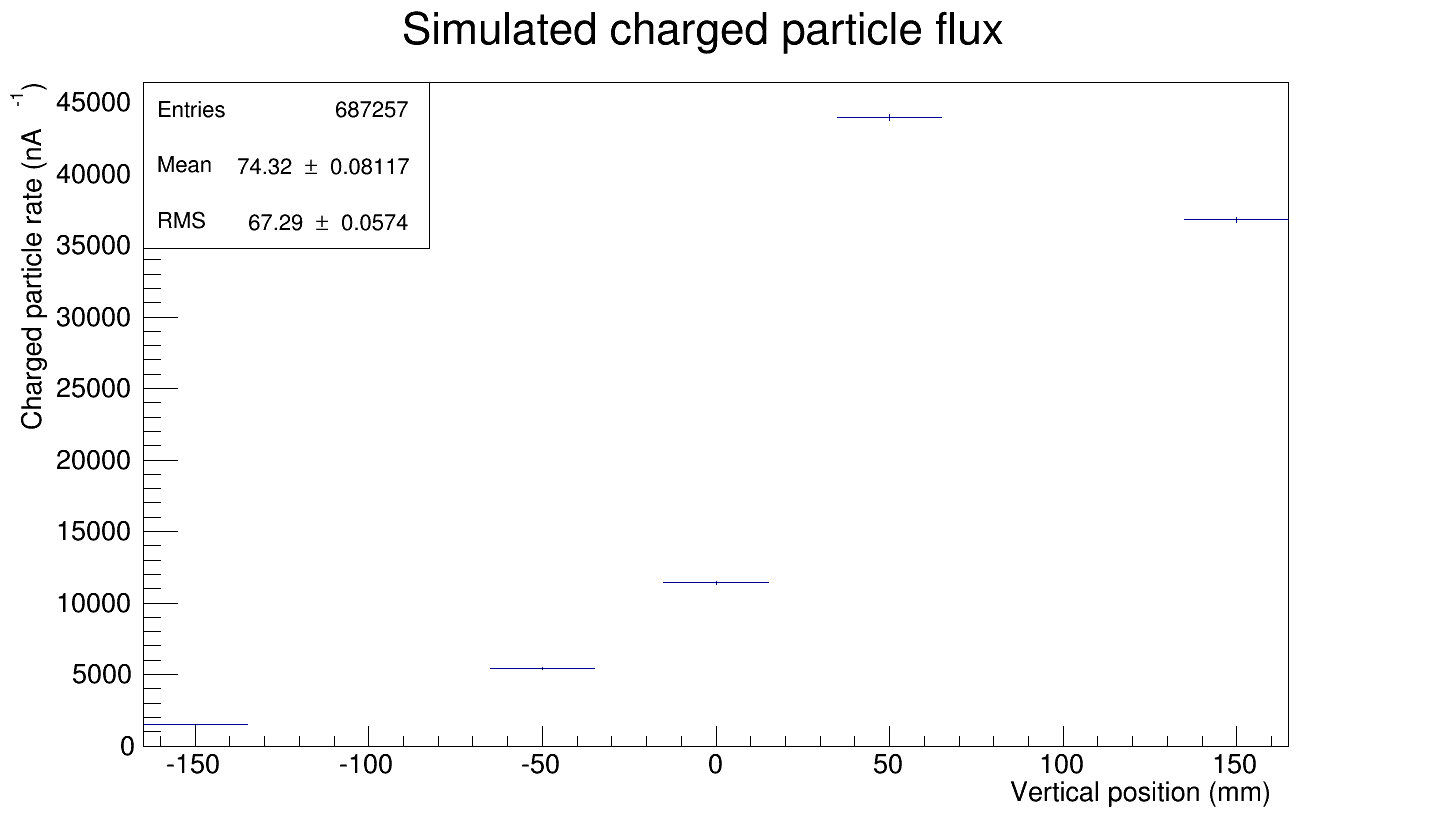
\includegraphics[width=.9\textwidth]{images/plot_generating_scripts/sim_1d_charged_flux.png}
%   \caption{Simulated results for the 1D charged particle rate, normalised to a proton current of 1~nA. Values calculated as the un-adjusted number of charged particles in the 1D scintillator volume from \( 9\times10^8 \) initial protons generated in G4BL.}
%   \label{fig:sim_1d_charged_flux}
% \end{figure}
\begin{figure}[hptb]
  \centering
    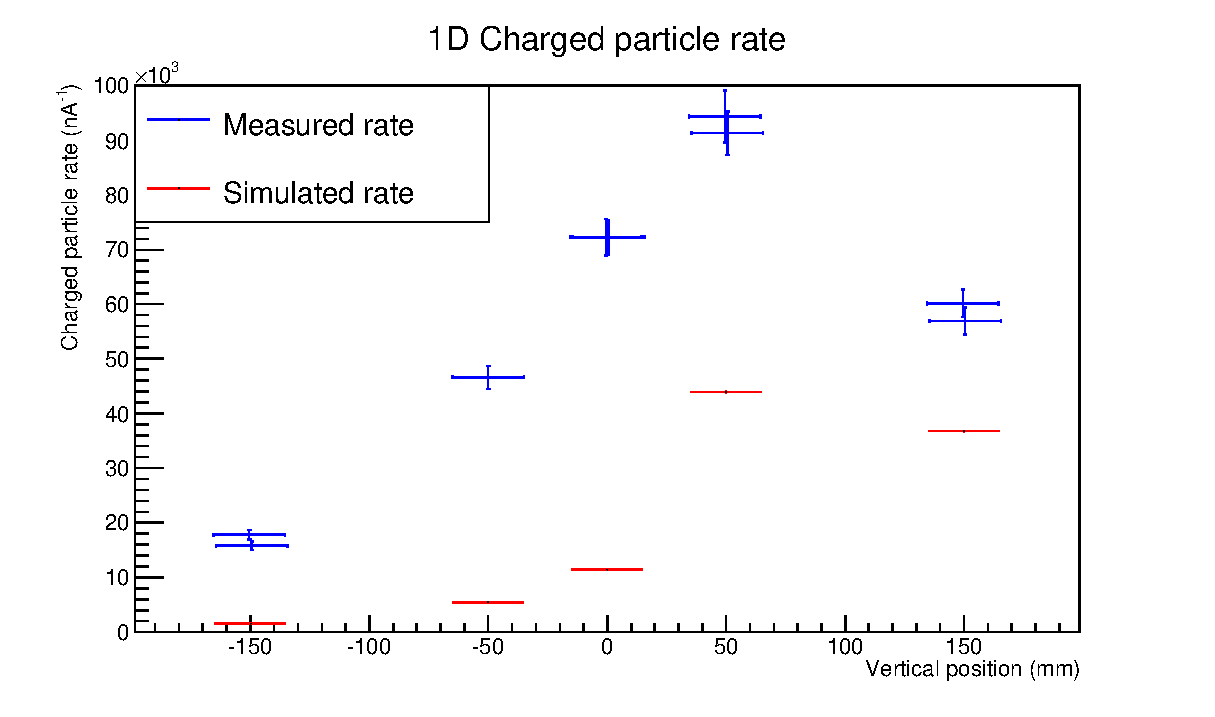
\includegraphics[width=.9\textwidth]{images/plot_generating_scripts/1D_charged_particle_flux.eps}
  \caption{Comparison of simulated and measured total charged particle flux.}
  \label{fig:images_plot_generating_scripts_1D_charged_particle_flux}
\end{figure}
  
\begin{figure}[hptb]
  \centering  
    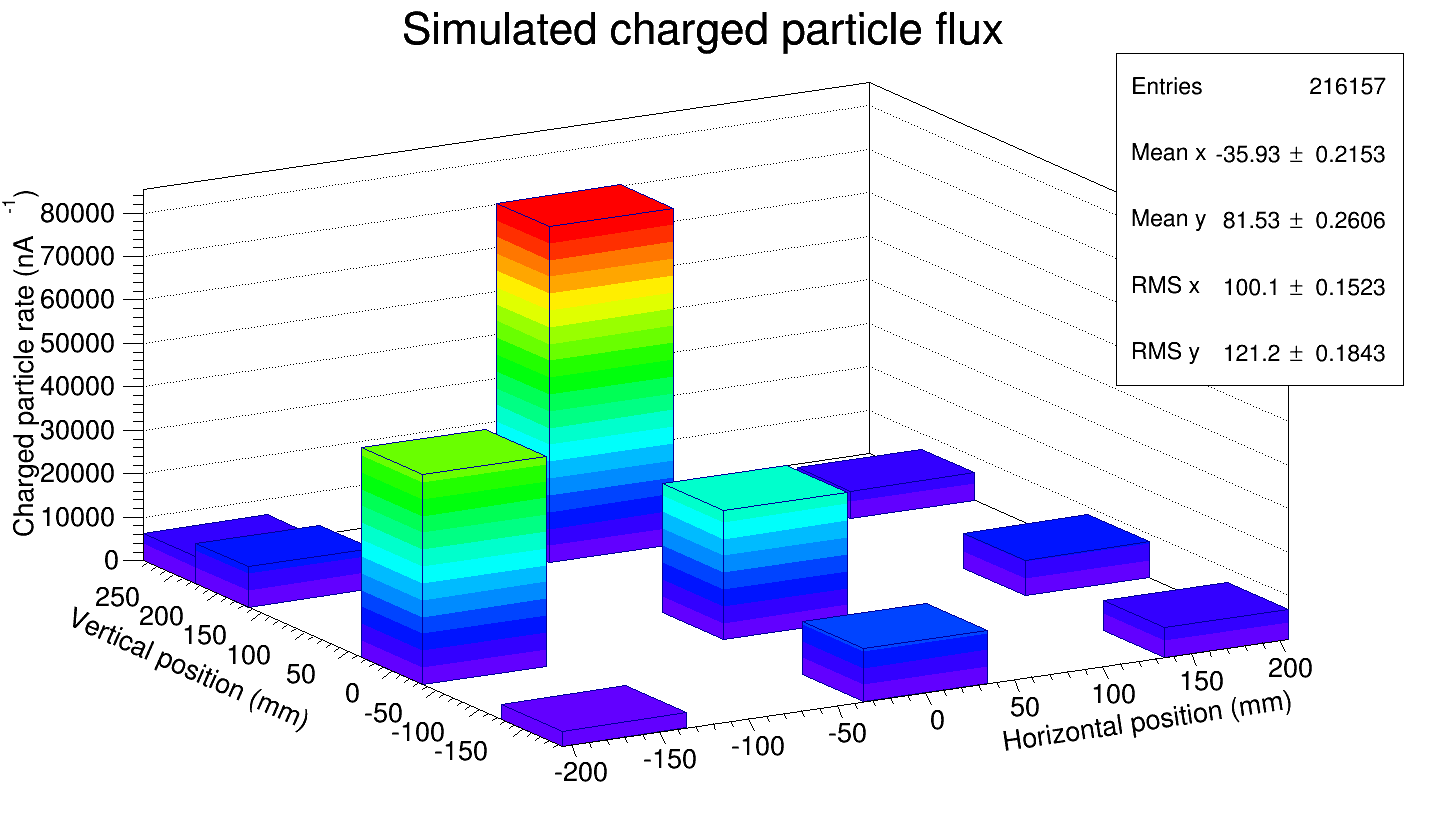
\includegraphics[width=.9\textwidth]{images/plot_generating_scripts/sim_2d_charged_flux.png}
  \caption{Simulated results for the 2D charged particle rate normalised to a proton current of 1~nA. Colour is equal to the rate as given by the z-axis. Simulated using \( 9\times10^8 \) in G4BL, the rate was taken to be those particles seen within the area of the scintillator used.}
  \label{fig:sim_2d_charged_flux}
\end{figure}

% section analysis (end)
% chapter charged_particle_flux (end)
\section{Muon Lifetime} % (fold)
\label{cha:muon_lifetime}
Measurement of the muon lifetime is primarily used as a basic form of particle identification. Muons have a relatively long lifetime (\(2.197~\mu\)s) that acts as a useful method of identification. Measuring the muon lifetime is also a reasonably simple measurement that can be made with basic equipment. Two scintillators are placed on either side of a suitable stopping target along the muon's direction of travel. The muons loose energy as they traverse the stopping target and some number will stop, these can then be detected by the electrons produced in their decay. Plotting the differences in time between a detection at the upstream scintillator and the downstream scintillator will then produce the characteristic exponential decay curve that can be used to measure the muon lifetime. The curve produced is actually the sum of two separate decay curves: the decay of free muons and, as we have a beam containing negative muons as well, a component due to negative captured muon decay. The ratio of these two component can be used to estimate the ratio of muon types within the beam.

In total three measurements of the muon lifetime were taken: one con-currently with the 2D charged particle flux measurement, a high-statistics run and then measurements that form the basis of the muon momentum spectrum measurement. The first two of these measurements will be discussed here and the final will be discussed in the final chapter of this part.

\subsection{Experimental Set Up} % (fold)
\label{sec:experimental_set_up}
The basic experimental set up for muon lifetime measurement has already been discussed: two scintillators sandwiching a stopping target. Both measurements were made using the same scintillator and stopping target: two \( 380\times50\times3.5 \)~mm scintillators and a \( 370\times80\times6 \)~mm pure copper target. Two MPPCs were mounted on the ends of each scintillator to provide readout. 

The DAQ used was a simple extension of the previous versions. This time, rather than measuring the time differences between the different individual MPPCs the TDC was used to measure the time between a hit on the upstream scintillator and then a hit on the downstream. A `hit' was considered to be a co-incident signal on both MPPCs of that scintillator. As a measure to reduce spurious signals due to other charged particles, e.g.\ electrons, a veto window of 50~ns was used. The veto window was a period following the upstream hit in which no hits were allowed in the downstream scintillator. The veto-window aimed to reject particles that didn't decay between the scintillators, unfortunately this removes a portion of the signal but enough remains for a reasonable measurement to be made.

% section experimental_set_up (end)
\subsection{Results} % (fold)
\label{sec:results} 
Figures~\ref{fig:music2_mu_lifetime} and \ref{fig:music3_muon_lifetime} shows the TDC measurements that were made to record the muon lifetime. The TDC bin values are converted to ns using:
\begin{align}
  t = K*(T_0-T)
\end{align}
where \( t \) is the real time, in ns, \( K \) is the calibration constant (0.025, measured by manufacturer), \( T \) is the value recorded in the MH-TDC and \( T_0 \) is the time when the start signal for the TDC was sent as recorded by the MH-TDC on a dedicated channel.

The data is then fitted with either one or two exponential decay functions and a flat background. Whether a single or double exponential is used depends heavily on the amount of data that was taken. A single function is mainly used to fit the free decay of muons whereas a second exponential can be used to model the decay of captured negative muons inside the stopping target. Fitting the copper-decay exponential requires much greater data as a significant proportion of the events from this are ignored because of the veto-window. In the first 50~ns \(\sim\)26~\% of all copper decays will have already occurred in comparison to only \(\sim\)2\% of free muon decays. 

\begin{figure}[hptb]
  \centering
  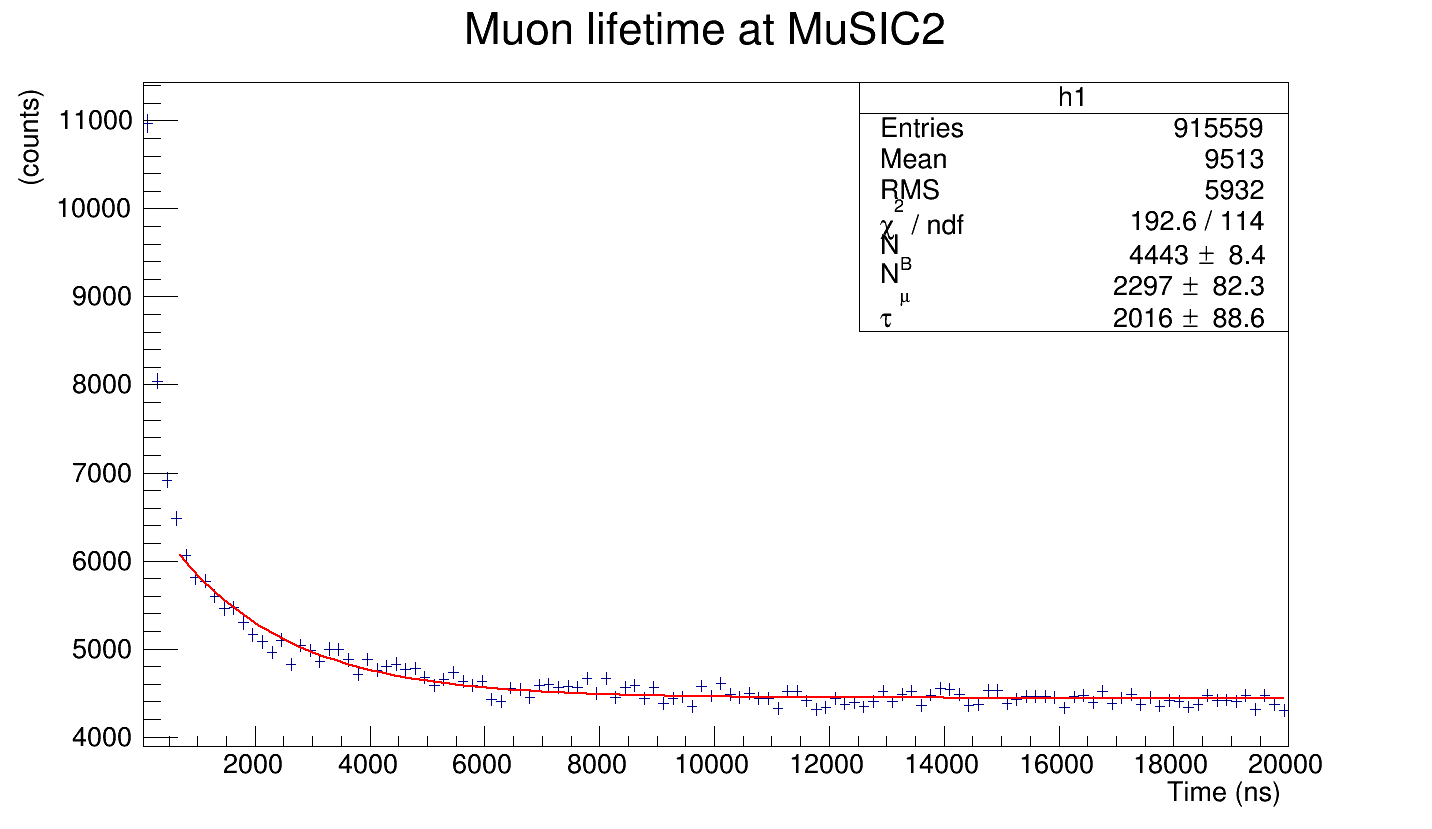
\includegraphics[width=.9\textwidth]{images/lifetime/music2_mu_lifetime_good.png}
  \caption{Results of the first measurement of the muon lifetime. The data was binned in 166~ns bins to remove the affects of noise on the data, only entries with an ADC value of 1,100 (which excluded the pedestal) were used.}
  \label{fig:music2_mu_lifetime}
\end{figure}
\begin{figure}[hptb]
  \centering
  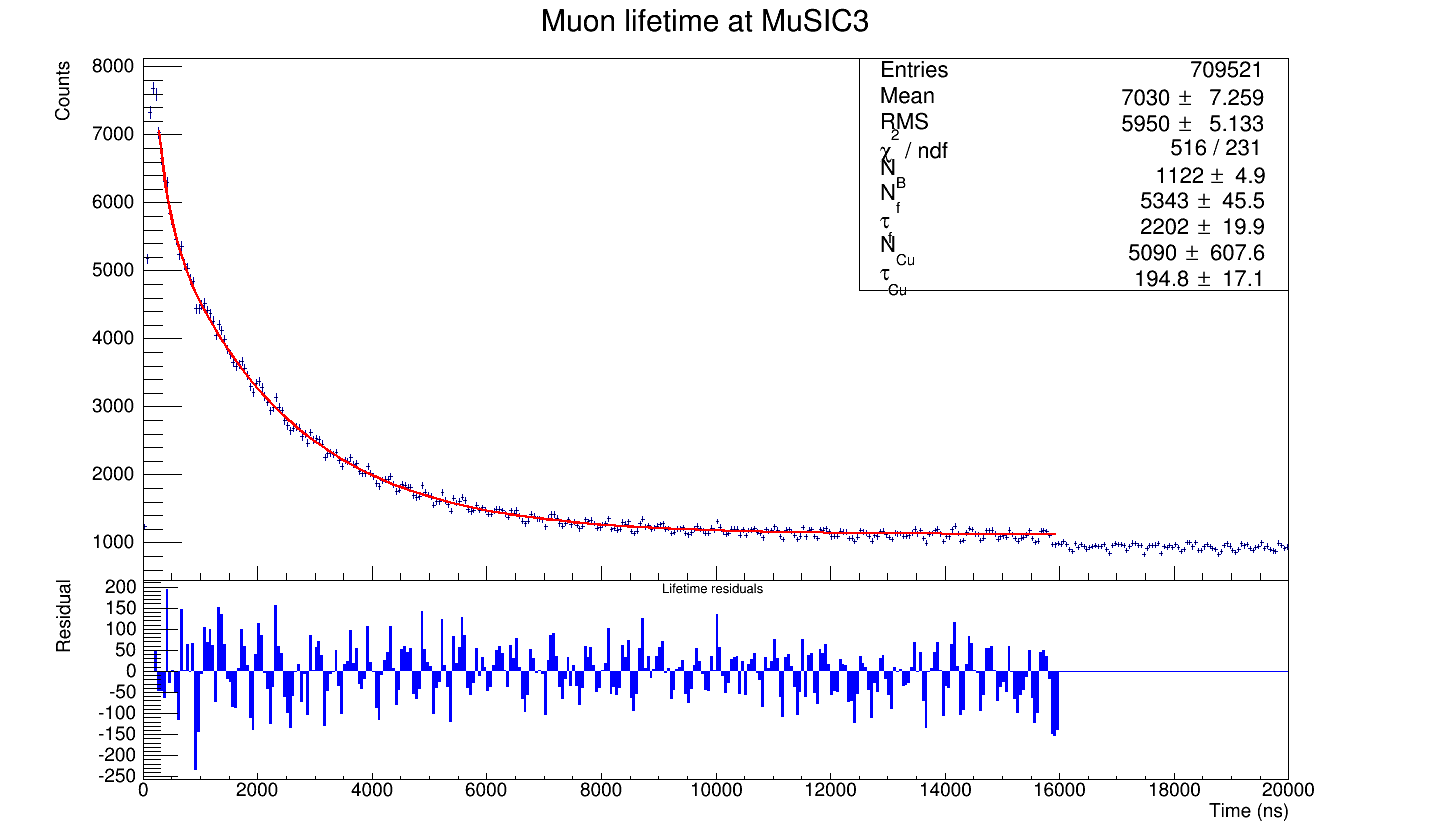
\includegraphics[width=.9\textwidth]{images/lifetime/music3_muon_lifetime.png}
  \caption{Results of the second measurement of them muon lifetime. The data was split between bins with a width of 480~ns and the data was fitted for values above 220~ns. The lifetime of muonic copper was fixed to \( 163.5\pm1.0 \)~ns.}
  \label{fig:music3_muon_lifetime}
\end{figure}

% section results (end)
\subsection{Analysis} % (fold)
\label{sec:analysis}
As can be seen in figures~\ref{fig:music2_mu_lifetime} and \ref{fig:music3_muon_lifetime} the exponential decays are good fits to the data with reasonable chi-squared values (\(192.6/114\) and \( 728.7/240 \) respectively). The muon lifetimes measured are in good agreement with the canonical value of \(2.1969811\pm0.0000022\)~\cite{PDG} although the MuSIC2 measurement. Both measurements are low (with the MuSIC2 measurement being significantly lower) but this should be due to affects of other materials in the detector, for example the plastic scintillator which has a captured muon lifetime of \(2026.3\pm1.5\)~ns~\cite{SUZUKI}. 

% section analysis (end)
% chapter muon_lifetime (end)
\section{Momentum Spectrum} % (fold)
\label{cha:momentum_spectrum}
The final experiment carried out at MuSIC that we will discuss is the measurement of the muon momentum spectrum. The experiment was also extended so that rather than a single narrow scintillator several scintillators forming a basic hodoscope were employed giving coarse vertical flux information as well the desired momentum measurements.

\subsection{Experimental Set Up} % (fold)
\label{sec:experimental_set_up}
To measure the muon momentum spectrum the detector had two separate problems to solve: how to identify muons and how to measure their momentum. Identification was carried out via extension of the previous techniques in measuring the muon lifetime, determination of the muon's momentum was done by using a degrader that masked the momentum properties of the beam hence allowing us to measure a narrow band of momenta. This section is split into two: first a discussion of the experimental set up and then a discussion of the DAQ system.

\subsubsection{Detector} % (fold)
\label{sub:detector}
The detector consisted of an aluminium degrader who's thickness could be varied to select different momentum ranges, a thin (0.5~mm) upstream counter and a thicker (3.5~mm) downstream counter on either side of a 0.5~mm copper stopping target. A schematic of the detector can be seen in figure~\ref{fig:m5_setup}. Based on simulation (PART~\ref{TBC}) we predicted the mean momentum of muons that decay for different degrader thicknesses, the momentum distributions for the muons that stop can be seen in figure~\ref{fig:stopped_muon_mom} whilst the initial muon momentum distribution is given in figure~\ref{fig:initial_muon_momentum}, the mean momentums are also tabulated in table~\ref{tab:stopped_muon_mom}.
\begin{figure}[htbp]
    \centering
        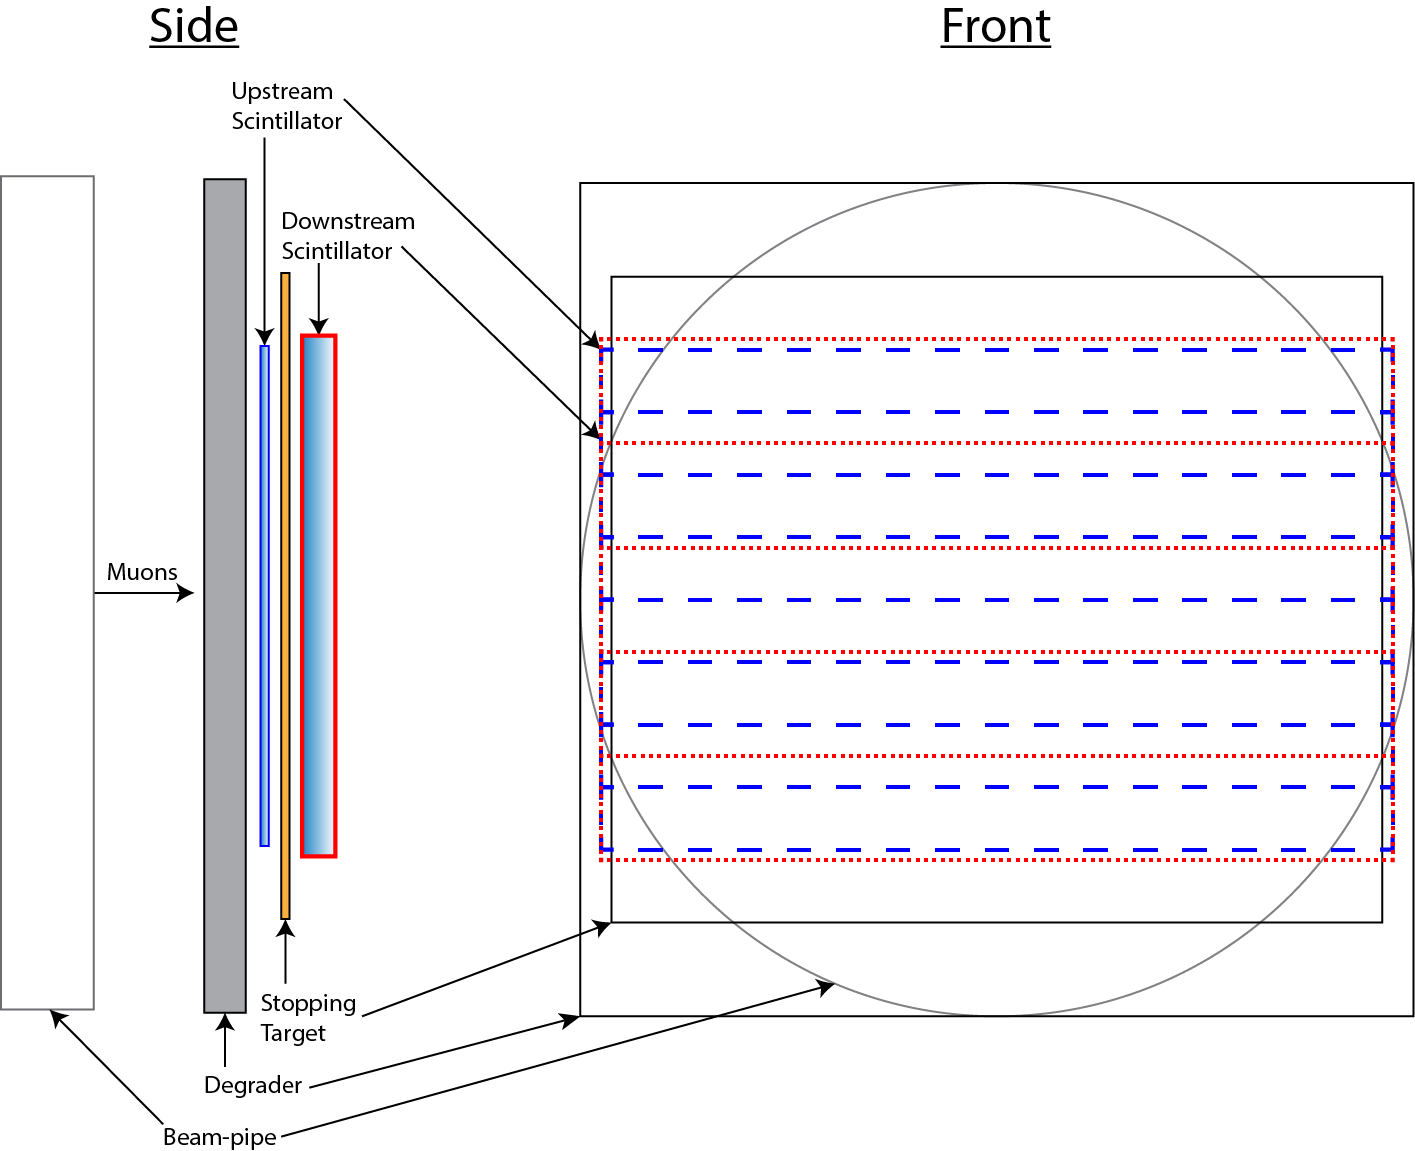
\includegraphics[scale=0.5]{images/momentum_spectrum/Detector_setup_music5.png}
    \caption{Experimental set up of the detector for MuSIC~5 (not to scale)}
    \label{fig:m5_setup}
\end{figure}  

The counters used were mylar wrapped scintillators with read-out performed by MPPCs mounted on either end of a wave length shifting fibre bounded along the long axis of the scintillator using optical cement. The signals from each pair of MPPCs are combined and amplified before being passed to the data acquisition system (DAQ) for processing.

Two important considerations were made with the chose of scintillators: the upstream scintillator had to minimise perturbation of the beam whilst providing a suitable trigger and the downstream scintillator had to be highly effective at detecting muons. To this end a thin (0.5~mm) upstream scintillator and thicker (3.5~mm) downstream scintillator were chosen. One downside of this set up is that in using a thin upstream scintillator the efficiency for detecting minimally ionising particles is reduced.

\subsubsection{Data Acquisition} % (fold)
\label{sub:data_acquisition}
The DAQ system used was a simple evolution of that used in the previous experiments: a discriminator unit with paired logic block formed a trigger on a suitably strong upstream signal with no downstream signal. The triggering signal was recorded using ADC and a MH-TDC was used to record hit times at the downstream scintillator within 20~\( \mu \)s of the trigger.

% The Data Acquisition (DAQ) took two measurements: the time at which signals arrived from the MPPC and the strength of those signals. The timing measurements are of the primary concern for this analysis. The DAQ itself had 3 distinct stages: discrimination, trigger formation and readout.
% 
% MPPCs are inherently noisy devices and discrimination is required to separate signal due to scintillation events from the MPPC's noise. A voltage threshold was set which (when exceeded) created a digital signal. Two thresholds were used: a lower one for the upstream counter and a higher one for the downstream counter. The lower threshold for the, thinner, upstream counters enabled better detection of minimally ionising muons whilst the higher downstream threshold enabled better detection of the more ionising electrons produced by muon decay. 
% 
% Using the signals from the discriminator a trigger was created based on the signature of muonic decay: the anti-coincidence of the up and downstream counters. It was assumed that a muon that doesn't decay in the detector region will be seen in both counters within a very small window of time ($<$50~ns). The only other constraint on the formation of a trigger was that the system wasn't busy in which case the trigger couldn't be accepted.

The trigger, once formed, signalled the start of readout. There were 3 modules to be read out via VMEbus (VME): a charge to Digital Converter (QDC), a scaler and a Multi-hit Time to Digital Converter (MTDC) which is of primary concern for this analysis. The MTDC recorded all signals  within a 20~\(\mu\)s period following the trigger that passed discrimination and that were anti-coincident with the other counter. Using a MTDC ensured that even if some beam remnant or dark event created a signal then the real signal would also be recorded and determined with background removal. The channel assignment used for the MTDC can be seen in table~\ref{tab:mtdc_ch}. To increase the accuracy of the MTDC the trigger time is recorded on a seperate channel called `TDC0'.
\begin{table}
    \begin{center}
    \begin{tabular}{c|c|c}
        Channel & Signal & Notes\\
        \hline
        0  & TDC0 & Time at which the trigger was formed \\
        \hline
        1  & U1   & \multirow{8}{*}{Upstream Counter}\\
        2  & U2   & \\
        3  & U3   & \\
        4  & U4   & \\
        5  & U5   & \\
        6  & U6   & \\
        7  & U7   & \\
        8  & U8   & \\
        \hline
        9  & D1   & \multirow{5}{*}{Downstream counter}\\
        10 & D2   & \\
        11 & D3   & \\
        12 & D4   & \\
        13 & D5   & \\
        \hline
        14 & Ge1  & \multirow{2}{*}{Germanium counter (not used in this analysis)}\\
        15 & Ge2  & \\
    \end{tabular}
    \end{center}
    \caption{Channel assignment for the MTDC. QDC channel assignment follows the same scheme but has no entry for channel 0 (as TDC 0 will be one of the upstream counters by design).}
    \label{tab:mtdc_ch}
\end{table}

A scaler was used to record system diagnostics (e.g. the trigger rate) by polling the scaler regularly during each run. The QDC recorded the strength of the trigging signal by integrating its charge over 100~ns. This information has not be incorporated into the current analysis but may be used in later analysis, for example to apply more stringent energy cuts at trigger time or for selection of regions of interest. The QDC had the same channel assignment as the TDC but without the germanium detector (as it had its own analogue to digital converter) and TDC0 (which was a digital signal).
\begin{table}
    \centering
    \begin{tabular}{c|c|l}
        Channel & Signal & Notes\\
        \hline
        0 & SEC & Measure of the proton current\\
        1 & Trigger & number of t0's\\
        2 & U and $\overline{\text{D}}$ & count of potential triggers\\
        3 & U & Upstream only\\
        4 & D & Downstream only\\
        5 & Scint & -\\
        6 & unused & -\\
        7 & clk & Record of time passed\\
    \end{tabular}
    \caption{Table of scaler channels and their designation}
    \label{tab:scaler_chs}
\end{table}

% subsection data_acquisition (end)
% section experimental_set_up (end)
\subsection{Data Processing} % (fold)
\label{sec:run_data}
There are 5 stages in preparing the experimental data for analysis (receipt of the data from MIDAS, de-serialisation, calibration, restructuring and histogramming). These will will be explained in more detail in the following sub-sections but the general process will be discussed here. The first stage is the receipt of data from the DAQ via MIDAS, this creates files of raw data which has to be de-serialised in the next stage before having calibration applied to it. The final stages are to restructure the data according to channel and then create histograms of the TDC values ready for analysis. 

These processes are split across 4 programs: MIDAS; mu\_analysis and mid2root\_converter (which act on .root and .mid MIDAS files respectively); and finally tdc\_file.py which is a python script for creating the TDC histograms.

For the analysis 6 runs were chosen, all using the 0.5~mm copper stopping target. For 5 of the runs an aluminium degrader was used. The run information is summarised in table~\ref{tab:run_summary}.
\begin{table}
	\begin{center}
	\begin{tabular}{c|c|c|c}
		Run ID & Time (sec) & Current (pA) & Degrader (mm) \\
		\hline
		448    & 9,221      & 15           & 0.0   \\
		451    & 1,001      & 15           & 0.5   \\
		452    & 4,924      & 13           & 0.5   \\
		455    & 6,307      & 13           & 1.0   \\
		458    & 5,144      & 14           & 5.0   \\
		459    & 2,452      & 12           & 5.0   \\
	\end{tabular}
	\end{center}
	\caption{Summary of the runs selected for this analysis. The degrader used aluminium and the stopping target 0.5~mm copper.}
	\label{tab:run_summary}
\end{table} 
\subsubsection{Data from MIDAS} % (fold)
\label{sub:data_from_midas}
MIDAS is `a general purpose data acquisition system for small and medium scale experiments'~\cite{ritt2012midas} and is the primary interface to the DAQ via VME. 

MIDAS stored the raw data from each run as a single file either in its own binary xml format (.mid files) or in ROOT~\cite{Brun199781} format (.root). Data was read from the VME crate in two asynchronous modes: `Trigger' and `Scaler' each corresponded to a separate tree structure in the resulting file. The majority of the time the system operated in trigger-mode: whenever a trigger was formed the controlling PC was informed and once the data had been gathered readout of the MTDC and QDC occurred via the VME. Scaler mode occurred at regular intervals and consisted of reading the diagnostics data gathered by the scaler, this did not reset the module which continued to accumulate data. 

Each tree contained a branch per module being read, the trigger tree also had also branch for errors (named `ERR'). The branches all had the same structure: an integer that recorded the number of values read and an array of integers containing those values. For the scaler and QDC modules the number of values read out was the same for every trigger as both had a fixed number of channels and took one measurement on each. The MTDC had a variable number of values to read out as it could record multiple hits on each channel.
% subsubsection data_from_midas (end)
\subsubsection{De-Serialisation} % (fold)
\label{sub:de_serialisation}
The first raw data from MIDAS for the MTDC and QDC were serialised and mangled with the channel number this means that they require processing before the real values can be extracted. Below are brief summaries of the algorithms used to de-serialise the MTDC data (listing~\ref{lst:mtdc_algo}), for full listings, including de-serialisation methods for QDC, see appendix~\ref{app:deserialisation}.
%
\begin{listing}[htbp]
    \begin{minted}[gobble=4]{c++}
    tdc_value      =  raw_val & 0x001f ffff
    tdc_channel    = (raw_val & 0x03e0 0000) >> 21
    tdc_valid_read = (raw_val & 0xf800 0000) == 0x0
    \end{minted}
    \caption{Method for de-serialising CAEN V1290N~\cite{CAENV1290N} data}
    \label{lst:mtdc_algo}
\end{listing}
% subsection de_serialisation (end)
\subsubsection{Calibration} % (fold)
\label{sub:calibration}
The MTDC has a stated least significant bit resolution of \(\sim\)25~ps with a 21 bits of data per value, this gives a maximum value of 52~\(\mu\)s. Conversion from the stored value to real, trigger aligned, time is done using the formula:
\begin{align}\label{equ:tdc_calibration}
    t'   &= 0.024414(t - \text{TDC}0)
\end{align}
where $t'$ is the calibrated time, $t$ is the de-serialised MTDC value and TDC$0$ is the de-serialised trigger time. The value $0.024414$ is the calibration co-efficient as determined in Tran Nam's work~\cite{timecalibNam2012}
% subsection calibration (end)

\subsubsection{Restructure} % (fold)
\label{sub:restructure}
In order for the MIDAS data to be easily manipulated it was restructured. The initial format was a simple structure of one branch for each module (i.e. one for MTDC one for the QDC and a final one for errors). A second tree was used to store the scaler values. Each branch had a leaf for the number of values and a leaf with the array of values.

In the restructured file each channel is a branch of a tree with the following leaves: QDC, TDC0, nHITS, TDC[nHITS]. The QDC value is self-explanatory, TDC0 was the trigger time, nHITS was the number of entries recorded by the MTDC for that channel and TDC was an array of the values. The error data was ignored as was the scaler tree as these can be read from the original file if needed and neither was required for de-serialisation or calibration.
% subsection restructure (end)
\subsubsection{Histogramming} % (fold)
\label{sub:Histogramming}
Once the data has been restructured it is trivial to create a histogram of the TDC data for each channel which forms the basis of the later analysis. A basic bin width of 1~ns was used and a range from 0 to 20~\(\mu\)s. A time of 0 was used for the lowest bin as, although the data window began at 50~ns, the MTDC recorded data as a sliding window so some values prior to the trigger were also recorded. All the histograms for (i.e. for all channels for all runs) were saved in the same root file.
% subsection histogramming (end)
\subsection{Secondary calculations} % (fold)
\label{sec:secondary_calculations}
There are two secondary calculations that need to be performed to calculate the muon yield. These are the acceptance, the fraction of the total beam we can expect to detect, and the dead time, a measure of how much of the time the detector is unable to process new data due to being busy.
\subsubsection{Acceptance} % (fold)
\label{sub:acceptance}
To calculate the acceptance the ratio of initial muons to muons that passed a `trigger' cut was calculated. This is done by counting the number of muons in simulated G4BL output (section~\ref{sub:g4bl_particle_production}) and then using a macro similar to that used to digitise the simulation output (section~\ref{sub:digitisation_histogramming}) to mimic the triggering process.

The main difference between the acceptance macro (appendix~\ref{appsub:acceptance}) and the digitisation macro (appendix~\ref{appsub:digitisation_macro}) were in the cuts applied to select the particles. Rather than any possible parent particle in the upstream detector only muons are selected, similarly, in the downstream detector only electrons who had a parent muon are selected. A final requirement is that the time difference between muon and electron is greater than 50~ns.

The acceptance is then the ratio of muon/electron pairs to the initial number of muons:
\begin{align}
    \text{Acceptance} &= \frac{\text{Decay muons}}{\text{Initial Muons}} \label{equ:acceptance}
\end{align}
It is worth noting that given the above definition and method the acceptance changes due to the thickness and type of degrader used. Obviously a degrader that removed the majority of the muons from the beam will have a smaller acceptance as a smaller fraction of the beam will have survived to be detected. The results of the acceptance calculations are given in table~\ref{tab:acceptance}, the macro used can be seen in appendix~\ref{appsub:acceptance}.
\begin{table}
    \begin{center}
    \begin{tabular}{c| r@{ $\pm$ }l | r@{ $\pm$ }l | r@{ $\pm$ }l | r@{ $\pm$ }l }
        Degrader (mm) & \multicolumn{2}{|c}{Count (no cut)} &
                        \multicolumn{2}{|c}{Count ($\Delta t>50$~ns)} &
                        \multicolumn{2}{|c}{Initial Muons} &
                        \multicolumn{2}{|c}{Acceptance (\%)}\\
        \hline
              Air 5.0 & 6330 & 80 & 4540 & 67.4 & 95719 & 309.4 & 4.7 & 0.1\\
        Aluminium 0.5 & 5636 & 75 & 3999 & 63.2 & 95719 & 309.4 & 4.2 & 0.1\\
        Aluminium 1.0 & 5222 & 72 & 3689 & 60.7 & 95719 & 309.4 & 3.9 & 0.1\\
        Aluminium 5.0 & 3632 & 60 & 2472 & 49.7 & 95719 & 309.4 & 2.6 & 0.1\\
        
    \end{tabular}
    \end{center}
    \caption{The variance of acceptance with degrader thickness. In the final acceptance a cut on $\Delta t$ requiring it to be $>$50~ns was used to account for the anti-coincidence of the downstream counter. The number of initial muons is from the G4Beamline simulation.}
    \label{tab:acceptance}
\end{table}
% subsection acceptance (end)
\subsubsection{Dead time} % (fold)
\label{sub:dead_time}
The calculation of the dead time is unlike that of the acceptance as it was calculated based on the real data rather than simulation. Using the scaler it is possible to estimate how much of the time the DAQ was busy and hence what percentage of data was missed. 

As was stated in section~\ref{sub:data_acquisition} the scaler was used to record diagnostics on the DAQ. To calculate the dead time only two are needed, the trigger count and the potential trigger count which can be used to calculate the dead time thus:
\begin{align}
    D = \frac{\text{Potential Triggers}}{\text{Good Triggers}}
\end{align}
Where potential triggers are considered any anti-coincidence of the up without the downstream counter and a good trigger is one in which this occurs without the system being busy. The results for are given in table~\ref{tab:dead_time}. Obviously, the dead time is not used in the yield calculations using the simulated data.
\begin{table}
    \begin{center}
    \begin{tabular}{c|c|c|r@{ $\pm$ }l|r@{ $\pm$ }l|r@{ $\pm$ }l }
        Run & Degrader (mm of Al) & Run time (s) &
                              \multicolumn{2}{|c}{Good Triggers} &      
                              \multicolumn{2}{|c}{Potential Triggers} &
                              \multicolumn{2}{|c}{Dead time (\%)} \\
        \hline
        448 & 0.0 & 9221 & 9652965 & 3106 & 15678757 & 3959 & 61.57 & 0.03 \\
        451 & 0.5 & 1001 &  767321 & 875  &  1070366 & 1034 & 71.69 & 0.11 \\
        452 & 0.5 & 4944 & 3459886 & 1860 &  4667767 & 2160 & 74.12 & 0.05 \\
        455 & 1.0 & 6307 & 4090246 & 2022 &  5372409 & 2317 & 76.13 & 0.05 \\
        458 & 5.0 & 5144 & 2049077 & 1431 &  2454952 & 1566 & 83.47 & 0.08 \\
        459 & 5.0 & 2452 &  915314 & 956  &  1077534 & 1038 & 84.95 & 0.12 \\
    \end{tabular}
    \end{center}
    \caption{Dead time for each run along with the number of potential and good triggers. Run time is included to show the origin of the different counts.}
    \label{tab:dead_time}
\end{table}
% subsection dead_time (end)
\subsubsection{Gain stability} % (fold)
\label{sub:gain_stability}
In order to better understand possible sources of systematics in the experiment the total trigger rate for each run was plotted over time. The gain stability should then be proportional to this trigger rate, giving a measure of how well the detector was working and highlighting any possible problems in the run. To plot this value the events produced in a run were divided into 10 sections, each containing an equal number of events. Using the values recorded by the scaler the length of each section in seconds could be determined (channel 7, see table~\ref{tab:scaler_chs}) as could the number of triggers seen in that section (channel 1). The results are plotted in figure~\ref{fig:gain_stability}, note that as the degrader thickness is increased the fit value decreases which is consistent with fewer particles reaching the detector. Full listings for plotting the gain stability can be found in appendix~\ref{appsub:gain_stability}.
%

\begin{sidewaysfigure}
  % \begin{figure}%[htbp]
      \centering
          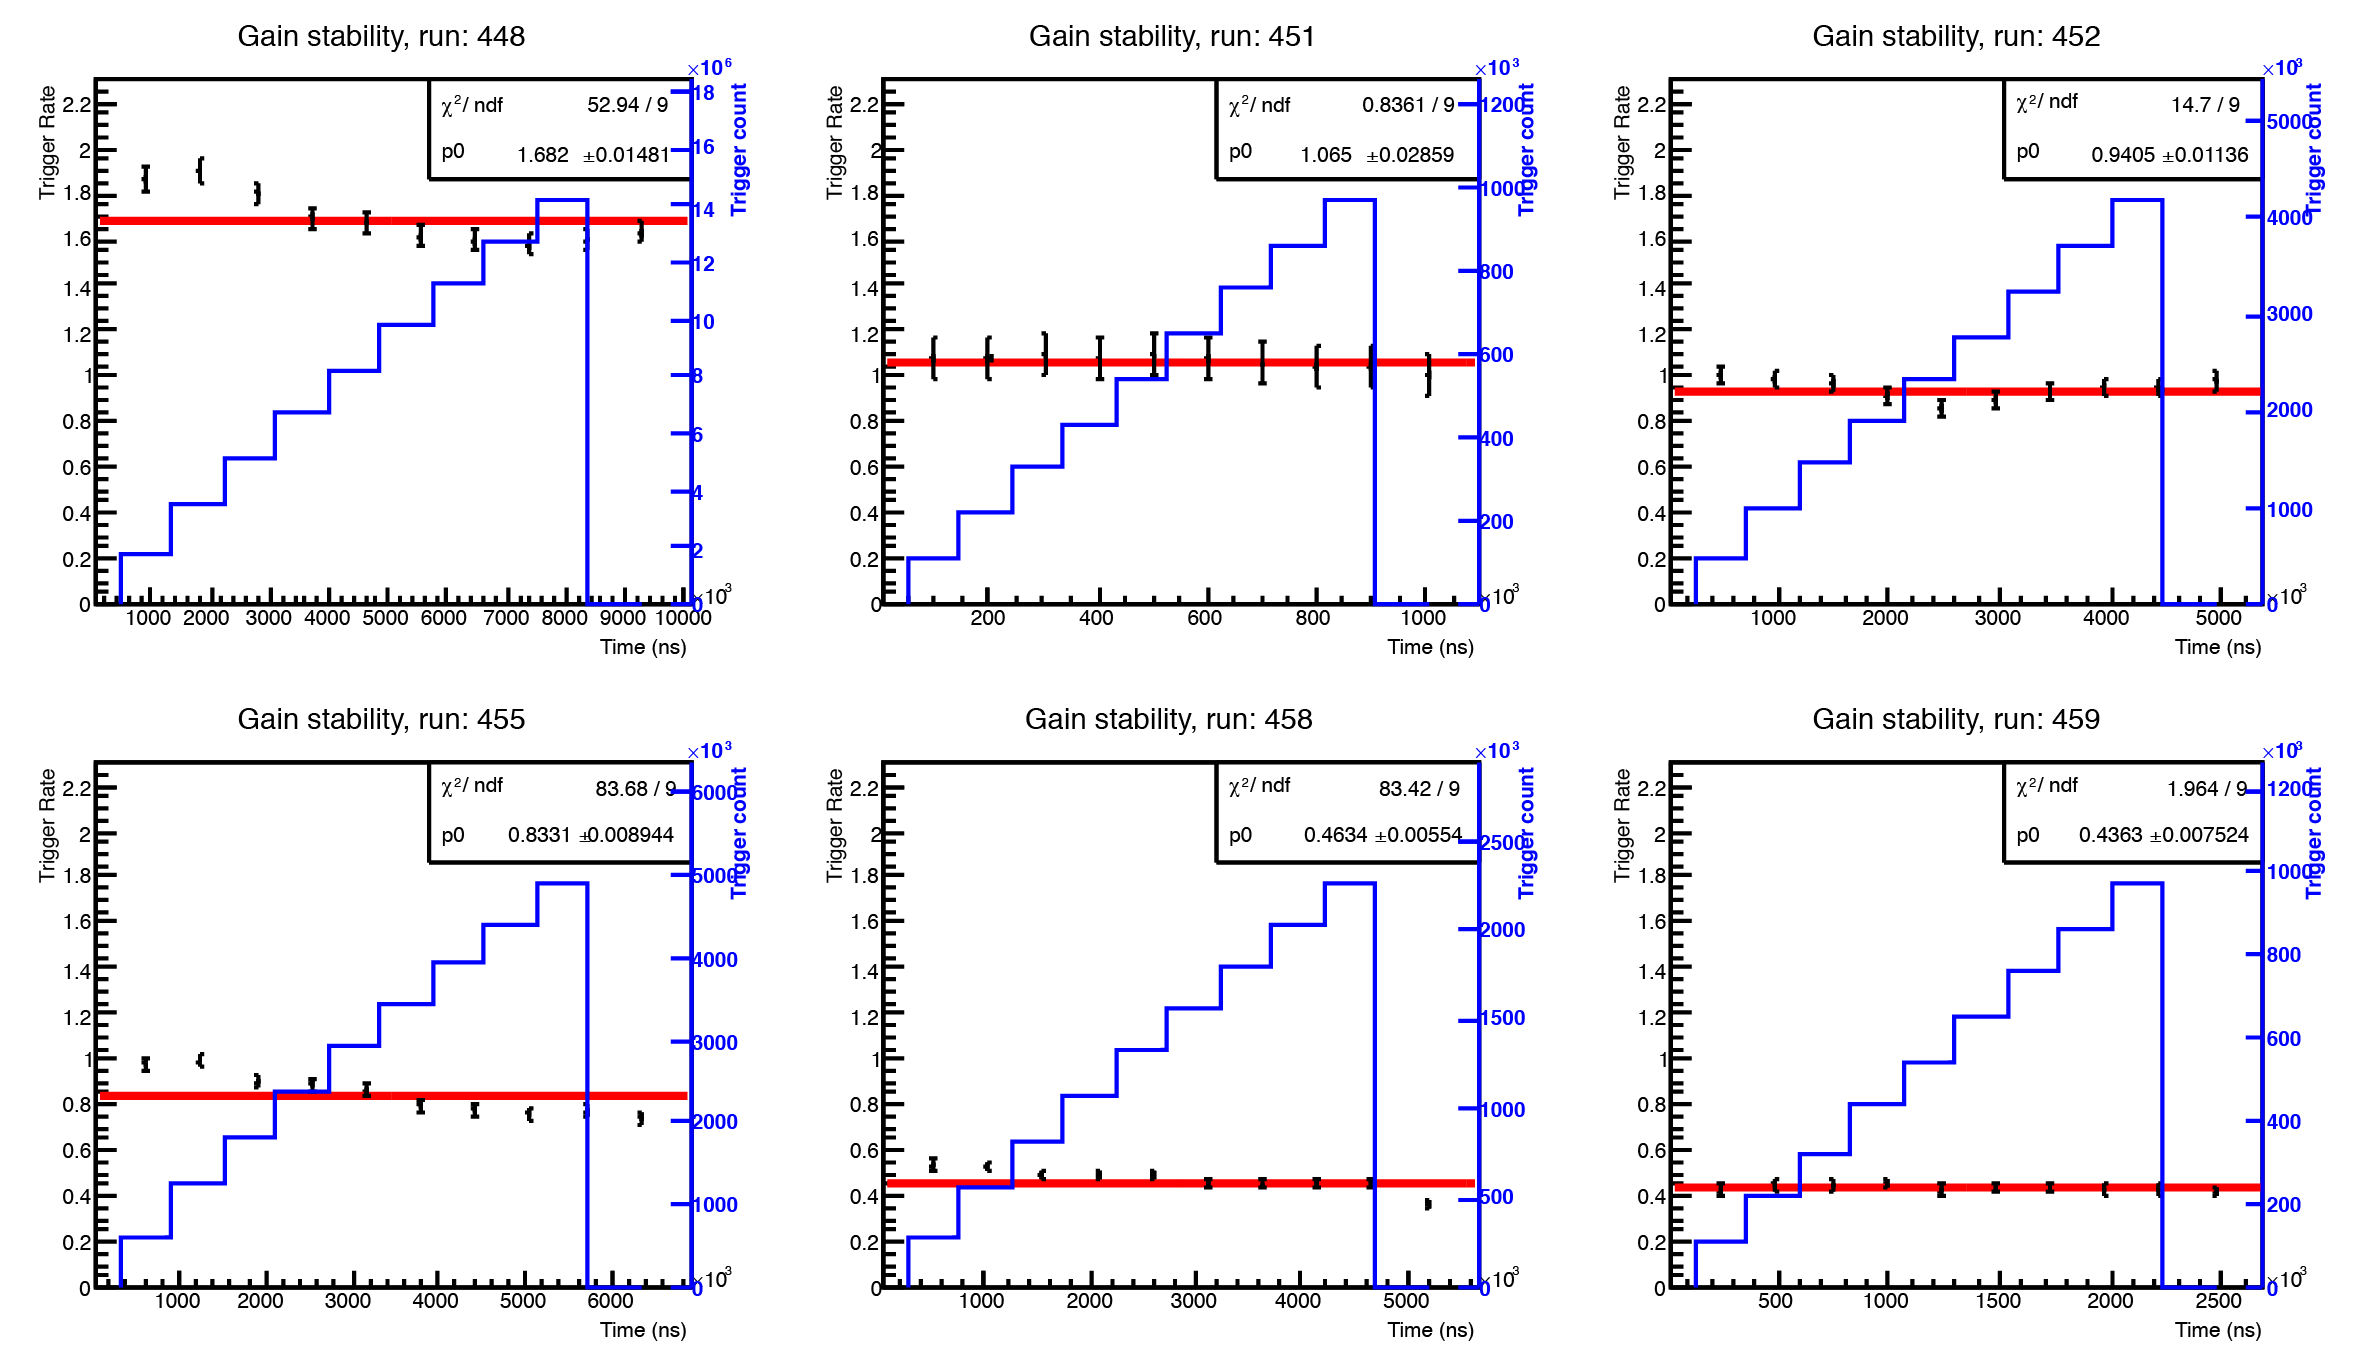
\includegraphics[width=\textwidth]{images/momentum_spectrum/gain_stability.png}
      \caption{Gain stability for each run, the black lines indicate the gain stability for that period of time (each is  \(\frac{1}{10}\) of the run) whilst the blue histogram plots the cumulative number of triggers. The gain stability has bit fitted with an order 0 polynomial who's parameters are given.}
      \label{fig:gain_stability}
  % \end{figure}
\end{sidewaysfigure}

%
\begin{table}
    \begin{center}
        \begin{threeparttable}
            \begin{tabular}{c|c|c|c|r@{ $\pm$ }l}
                Run & Al degrader thickness (mm) & $\chi^2$ 
                                                 & N.D.F. \tnote{a}
                                                 & \multicolumn{2}{|c}{Gain} \\
                \hline
                448  &  0.0  &  52.94   &  9  &  1.682  &  0.015  \\
                451  &  0.5  &  0.8361  &  9  &  1.065  &  0.029  \\
                452  &  0.5  &  14.7    &  9  &  0.940  &  0.011  \\
                455  &  1.0  &  83.68   &  9  &  0.8331 &  0.0089 \\
                458  &  5.0  &  83.41   &  9  &  0.4634 &  0.0055 \\
                459  &  5.0  &  1.964   &  9  &  0.4363 &  0.0075 \\
            \end{tabular}
            \caption{Gains as determined by the fits to the gain stability in figure~\ref{fig:gain_stability}.}
            \begin{tablenotes}
                \item [a] Number of Degrees of Freedom
            \end{tablenotes}
            \label{tab:gain_stability_paramters}
        \end{threeparttable}
    \end{center}
\end{table}

% subsection gain_stability (end)
% section secondary_calculations (end)
\subsection{Results} % (fold)
\label{sec:results}
As has been discussed there are 6 data sets that were used for this analysis, the details of them are given in table~\ref{tab:music5_run_summary}. For each run the TDC data was collected using the described method and calibrated. Each histogram was then fitted using the formula:
\begin{align}
  N_{f}\exp(\frac{-t}{\tau_{f}}) + N_{c}\exp(\frac{-t}{\tau_{c}}) + N_{s}\sin(2\pi\frac{t-\phi}{T}) + N_{b} \label{equ:fit}
\end{align}
Where the `\(N\)' terms are  scaling factors and `\(\tau\)' terms are lifetimes. The \(f\) terms refer to the free decay of muons; the \(c\) terms are muonic decays in copper; the \(s\) term is a sinusoidal source of noise with period \(T\) and phase \(\phi\), the \(b\) term is a constant background term.

Once the data was fitted using Root the \(f\) and \(c\) portions were integrated individually to calculate the number of free and copper decays the muons underwent. The fit results are shown in figures~\ref{fig:images_momentum_spectrum_448}~to~\ref{fig:images_momentum_spectrum_459} and summarised in table~\ref{tab:fit_res}. To improve the \(\chi^2\) values of the fits \(\tau_{f}\) and \(\tau_{c}\) were fixed at their given values of \(2,196.9811\pm0.0022 \)~ns~\ref{PDG} and \( 163.5\pm1 \)~ns~\ref{Suzuki Cu tau} respectively. The period, \(T\), was constrained to \(60\pm5\)~ns as this was determined to be a good value from fitting the noise (see figure~\ref{fig:images_momentum_spectrum_448_D1_noise_fit}). 

Fitting of the period of the background was done separately to the rest of the fit as this seemed to be something that ROOT struggled to do simultaneously with the other aspects of the fit. As can be seen a sinusoidal fit is not a very accurate description of the background but makes for a reasonable first-order approximation. 

In order to have good statistics whilst maintaining sensitivity to the relatively fast copper component of the decays a bin width of 16~ns was used. A large bin width (e.g.\ 100~ns) could have been used to smooth the sinusoidal noise but this would result in very few bins in which the copper component was significant. Whilst the ideal solution would be to use binning such that the sinusoidal component was cancelled out this was not feasible due to limitations of the fitting program. In the end a bin width was chosen that resulted in a small \(\chi^2\) whilst remaining sensitive to copper.

The number of muons was normalised between runs to the proton beam current using:
\begin{align}
  R &= \frac{N_{\mu}}{I_p D E} \label{equ:rate}
\end{align}
Where \( R \) is the normalised rate of muon decays (in nA\(^{-1}\)), \(N_{\mu}\) is the number of muon decays (either free or from muonic copper), \( I_p \) is the proton current in nA, \( D \) is the duration of the run in s and \( E \) is the dead time (as given in table~\ref{tab:dead_time}). The rates and number of muon decays are given in table~\ref{tab:rates_res} along with the \(\chi^2\) values for each fit. Again the majority of the beam is clearly towards the top of the beam pipe as has previously been seen.

Figures~\ref{fig:images_momentum_spectrum_run_muon_rate_in_f}~and~\ref{fig:images_momentum_spectrum_run_muon_rate_in_cu} show the rates of decays from free muons and muonic copper respectively. These plots are the `pure' rates based solely on the measured values. Between the pairs of runs (e.g.\ runs 451/452 and 458/459) there is good agreement and the general shape suggests that (unsurprisingly) as larger degraders are used there are fewer decays of stopped muons. As can be seen Further refinements can be made to enable more accurate comparison to simulation: inclusion of the acceptance and the detector efficiency as well as conversion of the degrader thickness to the simulated average momentums.

As can be seen in the fit data the \(\chi^2\) values for the fitting of channels D4 and D5 are generally poor because of this they were removed from the final, summed, rate calculation. The main cause of the poor \(\chi^2\) value is likely the low statistics compounded by the fact that, as the counters share a common trigger those scintillators that are further away from the beam spot will record a greater fraction of noise. Also clear is that even for the channels with better \(\chi^2\) values equation~\eqref{equ:fit} is not a full description of the data. This affect can be seen more clearly when the values for \( \tau_c \) and \( \tau_f \) are also fitted using ROOT, as shown in figures~\ref{fig:images_plot_generating_scripts_per_ch_copper_lifetime} and~\ref{fig:images_plot_generating_scripts_per_ch_free_lifetime} respectively. Both of these plots show that ROOT moves the fit away from the canonical values whilst simultaneously providing a worse \(\chi^2\) than is seen with the constrained values.

\begin{table}
  \begin{center}
  \begin{tabular}{c|c|c|c}
    \multirow{2}{*}{Run ID}  &  Degrader  &  Time  &  Proton Current  \\
                             &   (mm)     &   (s)  &   (pA)           \\
    \hline
    448  &  0.0   &   9221  &  15  \\
    451  &  0.5   &   1001  &  15  \\
    452  &  0.5   &   4944  &  13  \\
    455  &  1.0   &   6307  &  13  \\
    458  &  5.0   &   5144  &  14  \\
    459  &  5.0   &   2452  &  12  \\
  \end{tabular}
  \end{center}
  \caption{Summary of the run conditions. The degrader was aluminium and the stopping target was fixed at 0.5~mm~copper.}
  \label{tab:music5_run_summary}
\end{table}

\begin{table}
  \lineup % enable \0, \- & \.
  \begin{center}
  \begin{tabular}{ c | c | r@{\(\,\pm\,\)}l | r@{\(\,\pm\,\)}l | r@{\(\,\pm\,\)}l | r@{\(\,\pm\,\)}l | r@{\(\,\pm\,\)}l }
  % \begin{tabular}{ c | c | S@{\(\pm\)}S | S@{\(\pm\)}S | S@{\(\pm\)}S | S@{\(\pm\)}S | S@{\(\pm\)}S }
    Run  
      &  Channel  
             & \multicolumn{2}{c|}{\(N_b\)} 
                                 &  \multicolumn{2}{c|}{\(N_s\)}
                                                     &  \multicolumn{2}{c|}{\(\phi\)}  
                                                                         & \multicolumn{2}{c|}{\( N_c \)}
                                                                                           &\multicolumn{2}{c}{\( N_f \)} \\
    \hline
    \multirow{5}{*}{448}
      &  D1  &  576.85\0& 0.80   &  121.10\0& 1.15   &   2.19 & 0.21    &   549\.\0& 31    &  1377.2\0& 5.7  \\
      &  D2  &  914.39\0& 1.0    &  197.28\0& 1.44   &  10.33 & 0.16    &  1524\.\0& 38    &  1937.2\0& 6.9  \\
      &  D3  &  164.22\0& 0.43   &   40.68\0& 0.63   &  18.22 & 0.36    &   592\.\0& 21    &   620.3\0& 3.4  \\
      &  D4  &   32.07\0& 0.19   &    6.89\0& 0.28   &  57.02 & 0.96    &   193\.\0& 11    &   172.8\0& 1.7  \\
      &  D5  &   27.79\0& 0.18   &    6.37\0& 0.26   &   4.31 & 0.94    &    24.8  &\07.8  &    91.1\0& 1.4  \\
    \hline
    \multirow{5}{*}{451}
      &  D1  &   39.55\0& 0.21   &    2.38\0& 0.31   &  25.3\0& 2.4     &    29.4  &\08.1  &   101.4\0& 1.5   \\
      &  D2  &   62.27\0& 0.26   &   17.74\0& 0.38   &  13.28 & 0.50    &   153\.\0& 11    &   178.2\0& 1.9   \\
      &  D3  &   11.52\0& 0.12   &    3.60\0& 0.17   &  20.4\0& 1.2     &    85.6  &\06.5  &    57.76 & 0.99  \\
      &  D4  &    2.18\0& 0.05   &    0.61\0& 0.08   &   6.5\0& 3.0     &    25.9  &\03.5  &    16.59 & 0.49  \\
      &  D5  &    1.97\0& 0.05   &    0.65\0& 0.07   &   8.7\0& 2.6     &     7.3  &\02.6  &     8.78 & 0.40  \\
    \hline
    \multirow{5}{*}{452}
      &  D1  &  161.25\0& 0.43   &   43.56\0& 0.61   &   4.08 & 0.31    &   208\.\0& 17    &   435.5\0& 3.1  \\
      &  D2  &  252.14\0& 0.54   &   71.73\0& 0.76   &  12.39 & 0.25    &   706\.\0& 23    &   789.9\0& 4.0  \\
      &  D3  &   46.29\0& 0.23   &   15.70\0& 0.34   &  19.82 & 0.55    &   335\.\0& 13    &   266.7\0& 2.1  \\
      &  D4  &    8.95\0& 0.11   &    2.49\0& 0.16   &   0.00 & 1.64    &   128.2  &\07.5  &    76.6\0& 1.1  \\
      &  D5  &    8.01\0& 0.097  &    2.37\0& 0.14   &   7.54 & 1.43    &    25.9  &\05.2  &    38.71 & 0.82  \\
    \hline
    \multirow{5}{*}{455}
      &  D1  &  187.67\0& 0.46   &   46.99\0& 0.66   &   4.38 & 0.32    &   265\.\0& 19    &   539.1\0& 3.4  \\
      &  D2  &  293.99\0& 0.58   &   73.76\0& 0.83   &  12.41 & 0.26    &   896\.\0& 26    &   967.9\0& 4.4  \\
      &  D3  &   54.02\0& 0.25   &   17.18\0& 0.37   &  20.27 & 0.53    &   438\.\0& 15    &   326.4\0& 2.3  \\
      &  D4  &   10.37\0& 0.11   &    2.86\0& 0.16   &   0.00 & 0.36    &   195.1  &\08.5  &    87.4\0& 1.1  \\
      &  D5  &    9.30\0& 0.10   &    2.63\0& 0.15   &   4.8\0& 1.3     &    41.9  &\05.8  &    47.00 & 0.90  \\
    \hline
    \multirow{5}{*}{458}
      &  D1  &   73.73\0& 0.29   &   21.53\0& 0.43   &   0.000 & 0.037  &   219\.\0& 15    &   350.2\0& 2.4  \\
      &  D2  &  114.37\0& 0.37   &   34.08\0& 0.54   &   5.32\0& 0.38   &   799\.\0& 20    &   562.4\0& 3.1  \\
      &  D3  &   21.47\0& 0.16   &    8.40\0& 0.24   &   9.89\0& 0.71   &   236\.\0& 11    &   178.1\0& 1.6  \\
      &  D4  &    3.805 & 0.070  &    1.25\0& 0.10   &   0.00\0& 0.19   &    72.6  &\05.8  &    49.23 & 0.80  \\
      &  D5  &    3.728 & 0.067  &    1.436 & 0.098  &   0.00\0& 0.76   &    19.1  &\04.2  &    28.11 & 0.65  \\
    \hline
    \multirow{5}{*}{459}
      &  D1  &   30.67\0& 0.19   &    8.86\0& 0.28   &  56.68 & 0.72    &   115.3  &\09.8  &   155.0\0& 1.6  \\
      &  D2  &   48.07\0& 0.24   &   14.91\0& 0.35   &   4.36 & 0.56    &   369\.\0& 13    &   254.0\0& 2.1  \\
      &  D3  &    8.87\0& 0.11   &    3.65\0& 0.16   &  11.3\0& 1.0     &   110.1  &\07.3  &    81.0\0& 1.1  \\
      &  D4  &    1.631 & 0.046  &    0.579 & 0.068  &  48.2\0& 3.1     &    39.2  &\04.9  &    22.01 & 0.54  \\
      &  D5  &    1.496 & 0.043  &    0.615 & 0.063  &   0.0\0& 1.0     &     8.0  &\02.8  &    12.73 & 0.43  \\
  \end{tabular}
  \end{center}
  \caption{Summary of the fitted values for equation~\eqref{equ:fit}. These are the values used for the calculation of the integrals and, ultimately, the muon rates. The two lifetime parameters, \( \tau_f \) and \( \tau_c \), were fixed at the values \(2,196.9811\pm0.0022 \)~ns~\ref{PDG} and \( 163.5\pm1 \)~ns~\ref{Suzuki Cu tau} respectively, \( T \) was fixed at 60~ns.}
  \label{tab:fit_res}
\end{table}

\begin{table}
  \lineup
  \begin{center}
  \begin{tabular}{c | c | r@{\(\,\pm\,\)}l | r@{\(\,\pm\,\)}l | r@{\(\,\pm\,\)}l | r@{\(\,\pm\,\)}l | r | l }
   \multirow{2}{*}{Run} 
     & \multirow{2}{*}{Channel}
          &  \multicolumn{2}{c|}{Copper}
                         &  \multicolumn{2}{c|}{Free}  
                                          & \multicolumn{2}{c|}{Rate (copper)}
                                                                 &\multicolumn{2}{c|}{Rate (free)}
                                                                     &\multicolumn{1}{c|}{\multirow{2}{*}{\(\chi^2\)}}
                                                                                     & \multicolumn{1}{c}{\multirow{2}{*}{NDF}}  \\ 
     &    & \multicolumn{2}{c|}{decays}
                         &  \multicolumn{2}{c|}{decays}  
                                           & \multicolumn{2}{c|}{(nA\(^{-1}\))}
                                                                & \multicolumn{2}{c|}{(nA\(^{-1}\))}
                                                                                     &         &      \\
   \hline
   \multirow{5}{*}{448}
     & D1 &   4098 & 232  &  184833 & 758  &    47.1\0& 2.7   &  2122.7  &  8.8   &    2772 & 1239  \\
     & D2 &  11377 & 286  &  259990 & 928  &   130.7\0& 3.3   &  2986\.\0& 11     &    5815 & 1239  \\
     & D3 &   4420 & 153  &   83253 & 458  &    50.8\0& 1.8   &   956.1  &  5.3   &    2116 & 1239  \\
     & D4 &   1462 &  85  &   23189 & 228  &    16.79 & 0.98  &   266.3  &  2.6   &  115129 & 1239  \\
     & D5 &    188 &  59  &   12223 & 183  &     2.16 & 0.68  &   140.4  &  2.1   &   37059 & 1239  \\
   \hline
   \multirow{5}{*}{451}
     & D1 &    220 &  60  &   13602 & 202  &    19.8\0& 5.4   &  1226\.\0& 18    &   2887 & 1239  \\ 
     & D2 &   1140 &  84  &   23915 & 261  &   102.8\0& 7.6   &  2155\.\0& 24    &   1592 & 1239  \\ 
     & D3 &    639 &  49  &    7751 & 132  &    57.6\0& 4.4   &   699\.\0& 12    &   1759 & 1239  \\ 
     & D4 &    193 &  26  &    2227 &  66  &    17.4\0& 2.3   &   200.7  &  6.0  &   3020 & 1239  \\ 
     & D5 &     55 &  19  &    1178 &  53  &     5.0\0& 1.8   &   106.1  &  4.8  &   2040 & 1239  \\ 
   \hline
   \multirow{5}{*}{452}
     & D1 &   1550 & 128  &   58446 & 413  &    32.2\0& 2.7   &  1214.5  &  8.6  &   1672 & 1239  \\
     & D2 &   5268 & 175  &  106013 & 538  &   109.5\0& 3.7   &  2203\.\0& 11    &   2416 & 1239  \\
     & D3 &   2501 & 100  &   35787 & 277  &    52.0\0& 2.1   &   743.6  &  5.8  &   1680 & 1239  \\
     & D4 &    957 &  57  &   10282 & 141  &    19.9\0& 1.2   &   213.7  &  2.9  &  32046 & 1239  \\
     & D5 &    196 &  39  &    5195 & 110  &     4.08 & 0.81  &   108.0  &  2.3  &   9906 & 1239  \\
   \hline
   \multirow{5}{*}{455}
     & D1 &   1976 & 142  &   72348 & 453  &    30.9\0& 2.2   &   1131.0 &  7.1  &   1766 & 1239  \\
     & D2 &   6689 & 194  &  129903 & 589  &   104.6\0& 3.0   &   2030.8 &  9.3  &   2726 & 1239  \\
     & D3 &   3273 & 112  &   43808 & 304  &    51.1\0& 1.8   &    684.9 &  4.8  &   1865 & 1239  \\
     & D4 &   1457 &  65  &   11730 & 151  &    22.8\0& 1.0   &    183.4 &  2.4  &  56096 & 1239  \\
     & D5 &    318 &  44  &    6308 & 121  &     4.97 & 0.69  &     98.6 &  1.9  &  15454 & 1239  \\
   \hline
   \multirow{5}{*}{458}
     & D1 &   1633 & 109  &   46999 & 328  &    27.9\0& 1.9   &    803.4 &  5.7  &   1418 & 1239  \\
     & D2 &   5968 & 149  &   75477 & 414  &   102.0\0& 2.6   &   1290.2 &  7.2  &   2265 & 1239  \\
     & D3 &   1765 &  82  &   23907 & 214  &    30.2\0& 1.4   &    408.7 &  3.7  &   1477 & 1239  \\
     & D4 &    542 &  44  &    6607 & 107  &     9.27 & 0.75  &    112.9 &  1.8  &  12516 & 1239  \\
     & D5 &    145 &  32  &    3773 &  87  &     2.48 & 0.54  &     64.5 &  1.5  &   5842 & 1239  \\
   \hline
   \multirow{5}{*}{459}
     & D1 &    861 &  74  &   20803 & 216  &    33.4\0& 2.9   &    806.5 &  8.5  &   1314 & 1239  \\
     & D2 &   2757 & 100  &   34085 & 275  &   106.9\0& 3.9   &   1321.4 & 10.8  &   1780 & 1239  \\
     & D3 &    822 &  55  &   10893 & 143  &    31.9\0& 2.1   &    422.3 &  5.6  &   1596 & 1239  \\
     & D4 &    293 &  37  &    2954 &  73  &    11.4\0& 1.4   &    114.5 &  2.8  &   3981 & 1239  \\
     & D5 &     61 &  21  &    1708 &  58  &     2.35 & 0.81  &     66.2 &  2.2  &   2110 & 1239  \\
  \end{tabular}
  \end{center}
  \caption{Summary of the results of integrating equation~\eqref{equ:fit} and using the values from table~\ref{tab:fit_res}. The rates are the initial values calculated using equation~\eqref{equ:rate}.}
  \label{tab:rates_res}
\end{table}

\begin{sidewaysfigure}
    \centering
      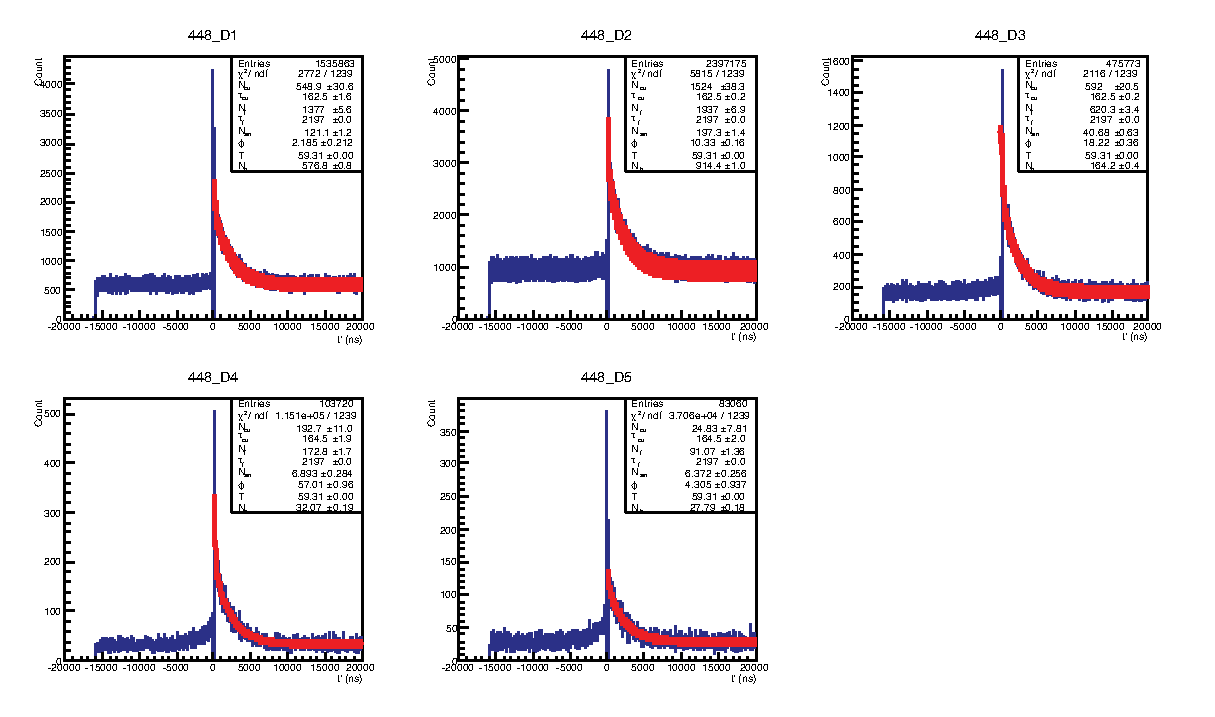
\includegraphics[scale=1]{images/momentum_spectrum/448.eps}
    \caption{Per channel fitting of data for run 448, for this run there was no degrader.}
    \label{fig:images_momentum_spectrum_448}
\end{sidewaysfigure}
%
\begin{sidewaysfigure}
    \centering
      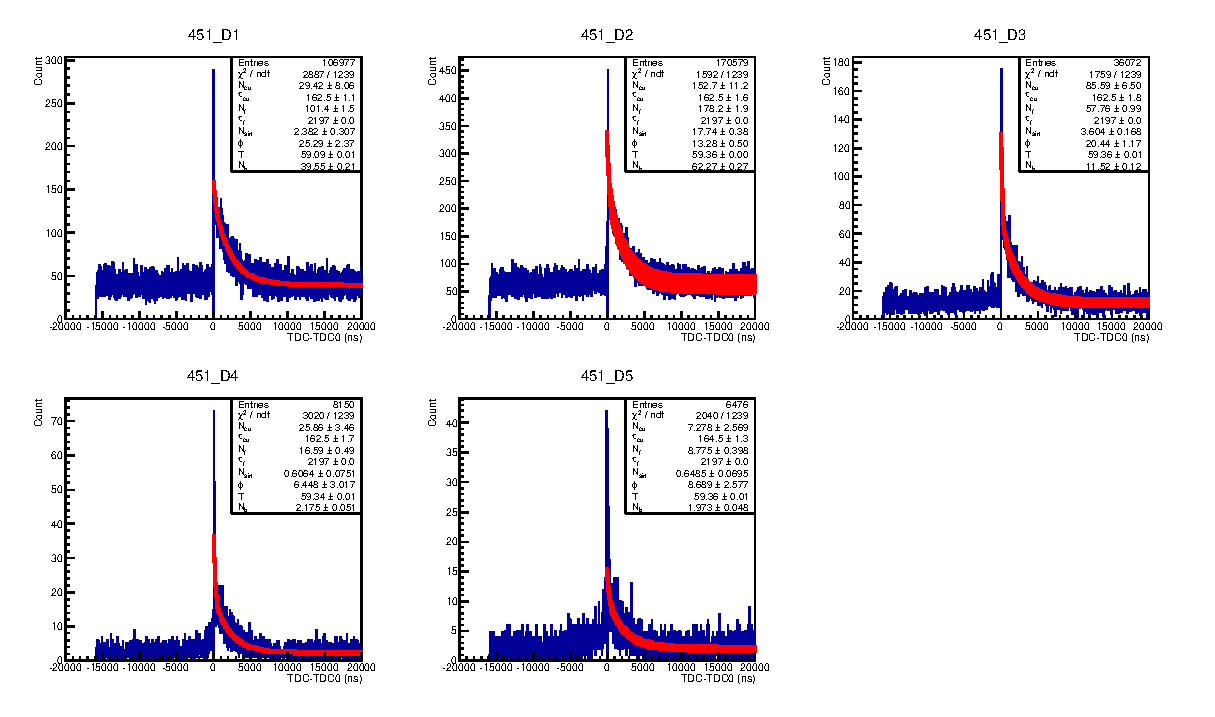
\includegraphics[scale=1]{images/momentum_spectrum/451.eps}
    \caption{Per channel fitting of data for run 451, for this run a 0.5~mm aluminium degrader was used.}
    \label{fig:images_momentum_spectrum_451}
\end{sidewaysfigure}
%
\begin{sidewaysfigure}
    \centering
      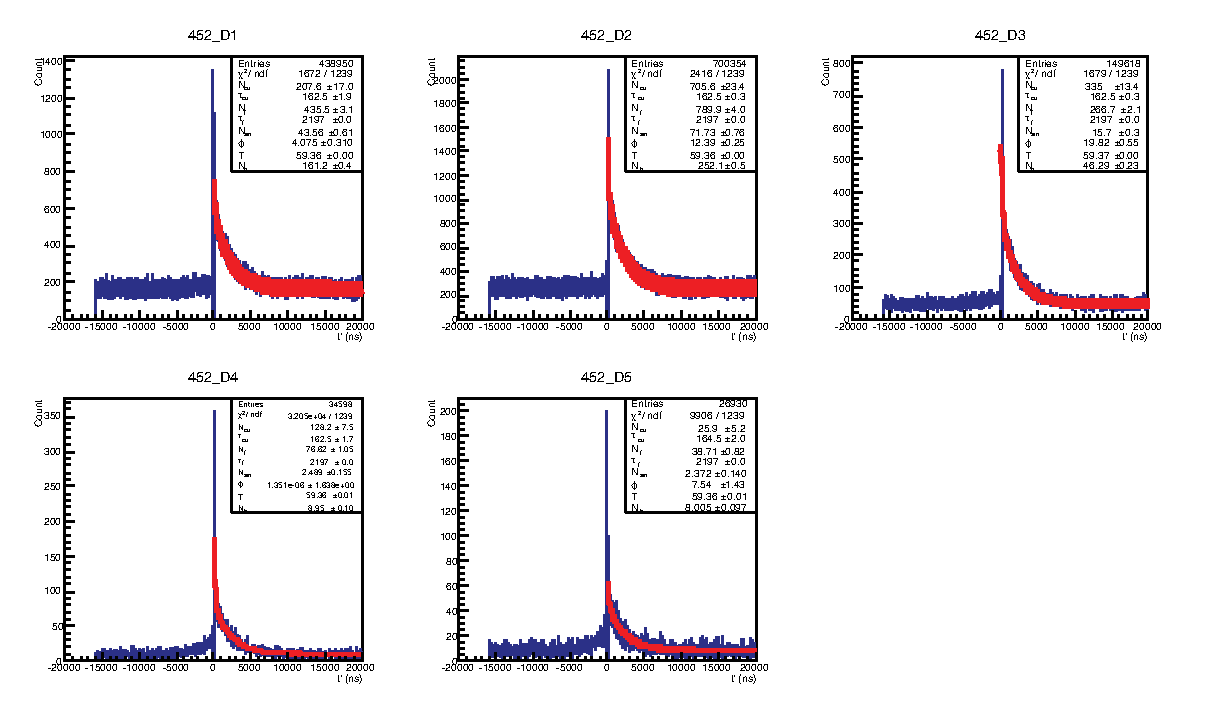
\includegraphics[scale=1]{images/momentum_spectrum/452.eps}
    \caption{Per channel fitting of data for run 452, for this run a 0.5~mm aluminium degrader was used.}
    \label{fig:images_momentum_spectrum_452}
\end{sidewaysfigure}
%
\begin{sidewaysfigure}
    \centering
      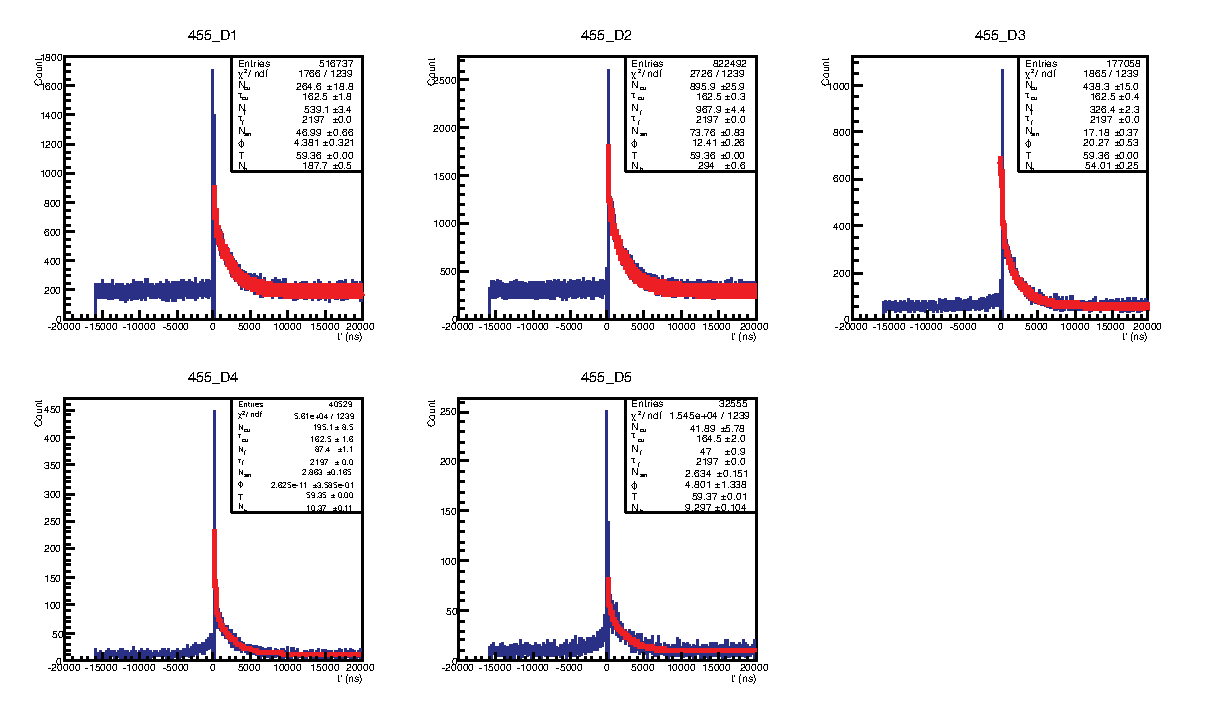
\includegraphics[scale=1]{images/momentum_spectrum/455.eps}
    \caption{Per channel fitting of data for run 455, for this run a 1~mm aluminium degrader was used.}
    \label{fig:images_momentum_spectrum_455}
\end{sidewaysfigure}
%
\begin{sidewaysfigure}
    \centering
      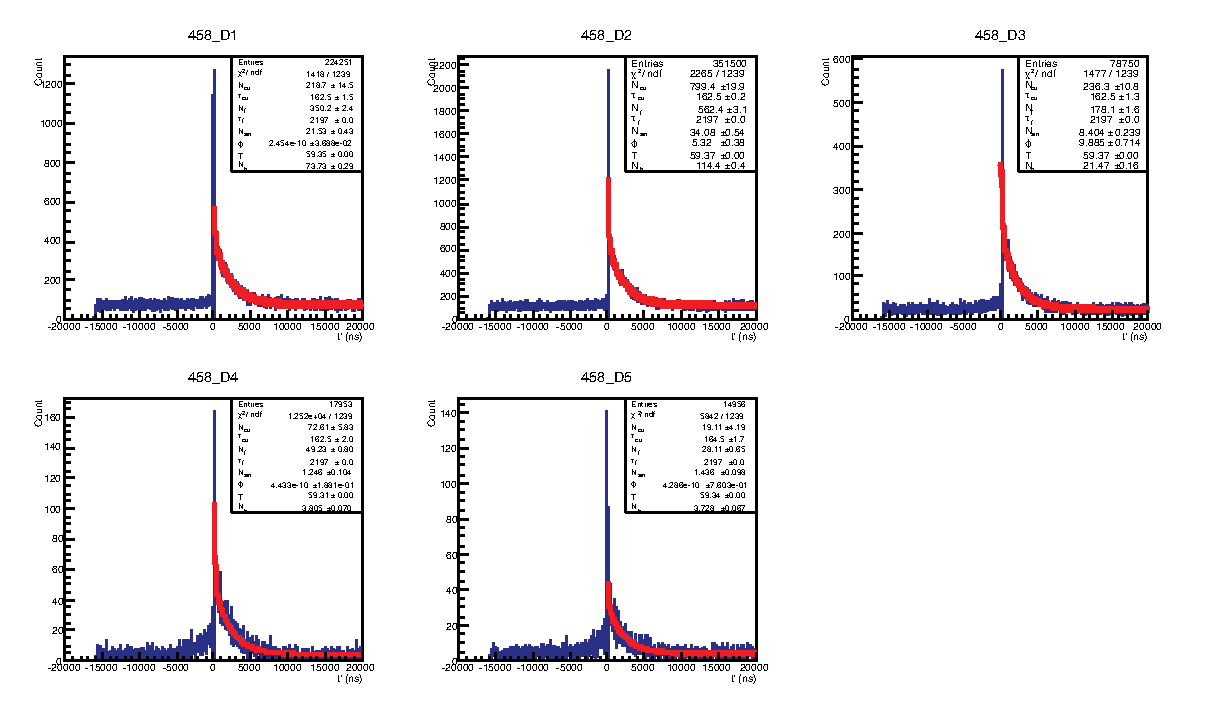
\includegraphics[scale=1]{images/momentum_spectrum/458.eps}
    \caption{Per channel fitting of data for run 458, for this run a 5~mm aluminium degrader was used.}
    \label{fig:images_momentum_spectrum_458}
\end{sidewaysfigure}
%
\begin{sidewaysfigure}
    \centering
      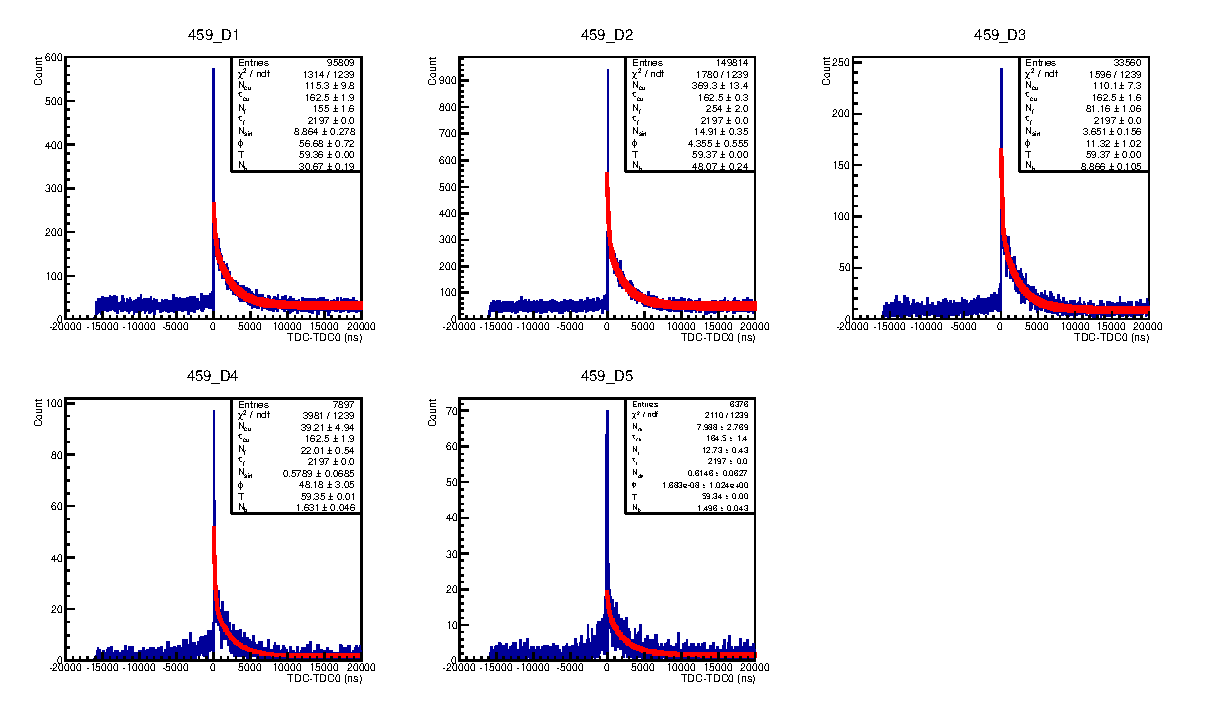
\includegraphics[scale=1]{images/momentum_spectrum/459.eps}
    \caption{Per channel fitting of data for run 459, for this run a 5~mm aluminium degrader was used.}
    \label{fig:images_momentum_spectrum_459}
\end{sidewaysfigure}

\begin{figure}[hptb]
  \centering
    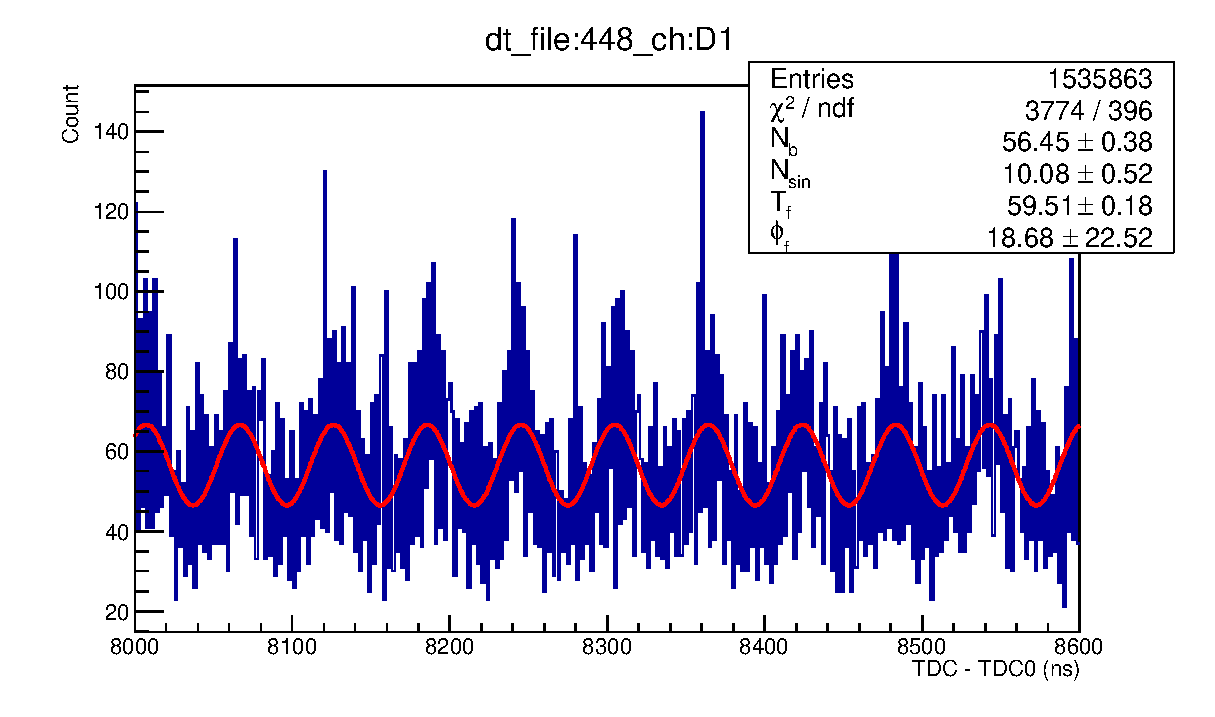
\includegraphics[width=.9\textwidth]{images/momentum_spectrum/448_D1_noise_fit.eps}
  \caption{Zoomed region (8,000~to~8,600~ns) of run 448, channel D1, showing the sinusoidal component of the background, the background has been fitted using \(N_b + N_s\sin(2\pi\frac{t-\phi}{T})\).}
  \label{fig:images_momentum_spectrum_448_D1_noise_fit}
\end{figure}

\begin{figure}[hptb]
  \centering
    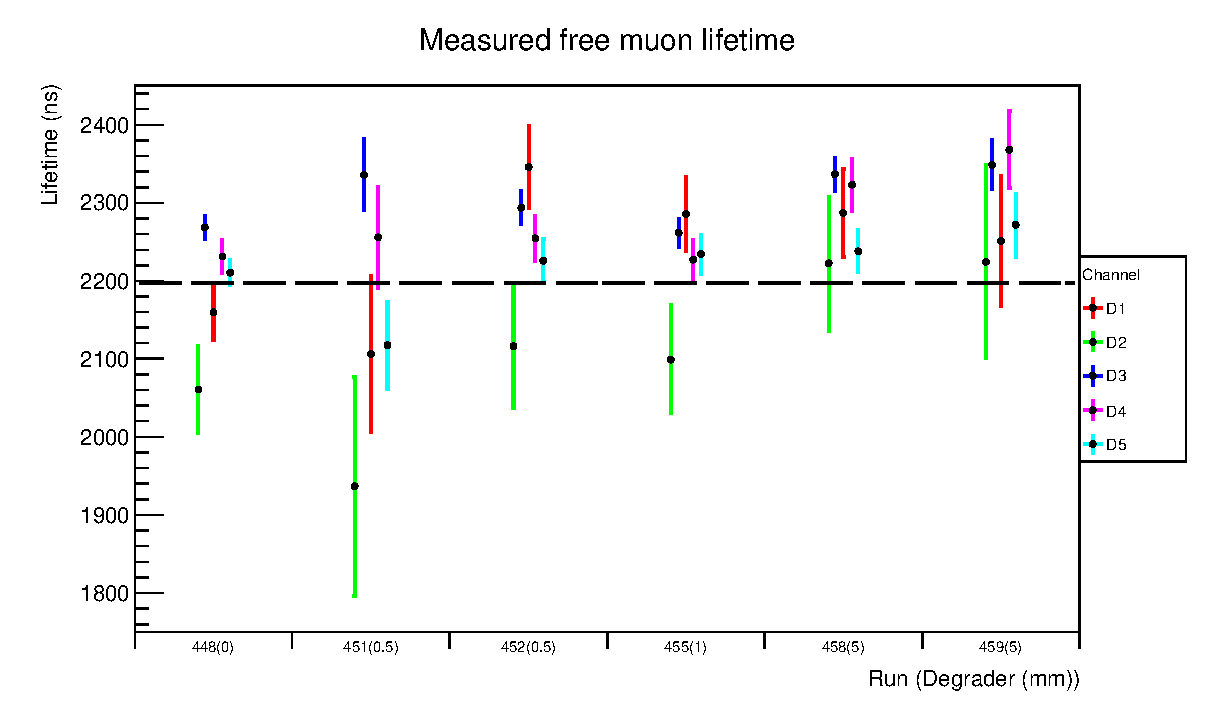
\includegraphics[width=.9\textwidth]{images/plot_generating_scripts/per_ch_free_lifetime.eps}
  \caption{Fitted values of free muon lifetime dependent on degrader and channel. The dashed line indicates the true value (\(2,196.9811\pm0.0022\)~ns~\ref{PDG}).}
  \label{fig:images_plot_generating_scripts_per_ch_free_lifetime}
\end{figure}
\begin{figure}[hptb]
  \centering
    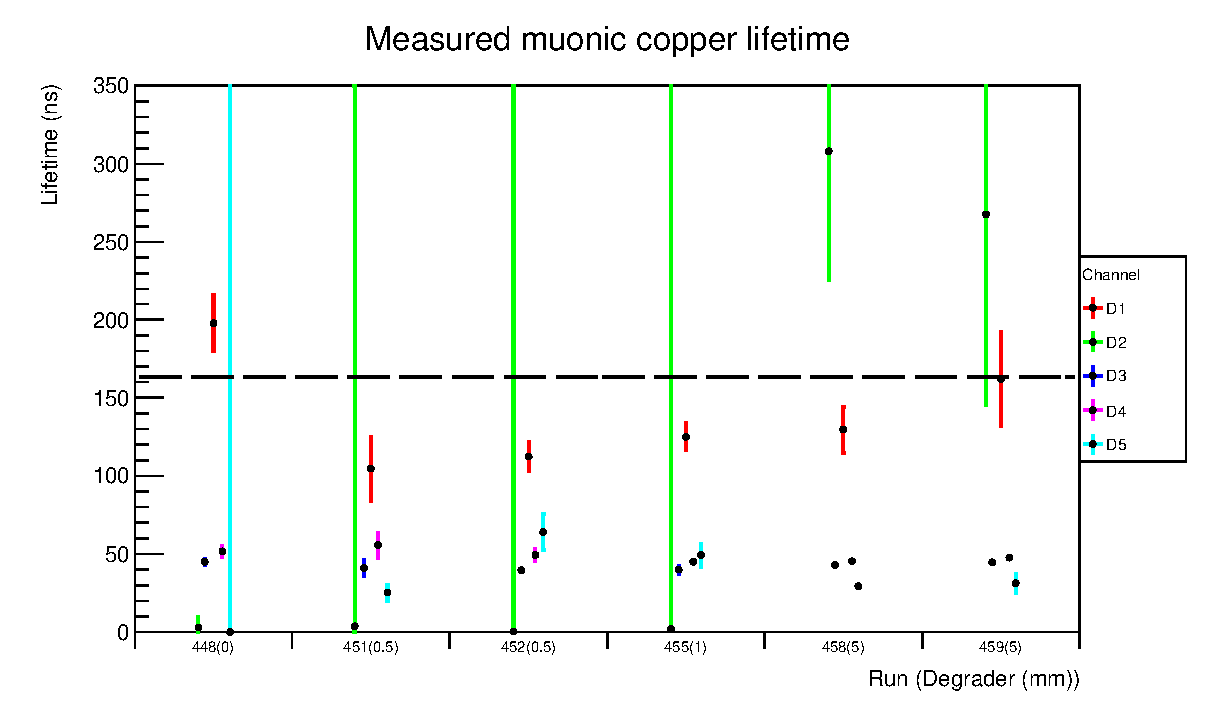
\includegraphics[width=.9\textwidth]{images/plot_generating_scripts/per_ch_copper_lifetime.eps}
  \caption{Fitted values of copper muon lifetime dependent on degrader and channel. The dashed line indicates the true value (\(163.5\pm1\)~ns~\ref{Suzuki cu tau}).}
  \label{fig:images_plot_generating_scripts_per_ch_copper_lifetime}
\end{figure}

\begin{figure}[hptb]
  \centering
    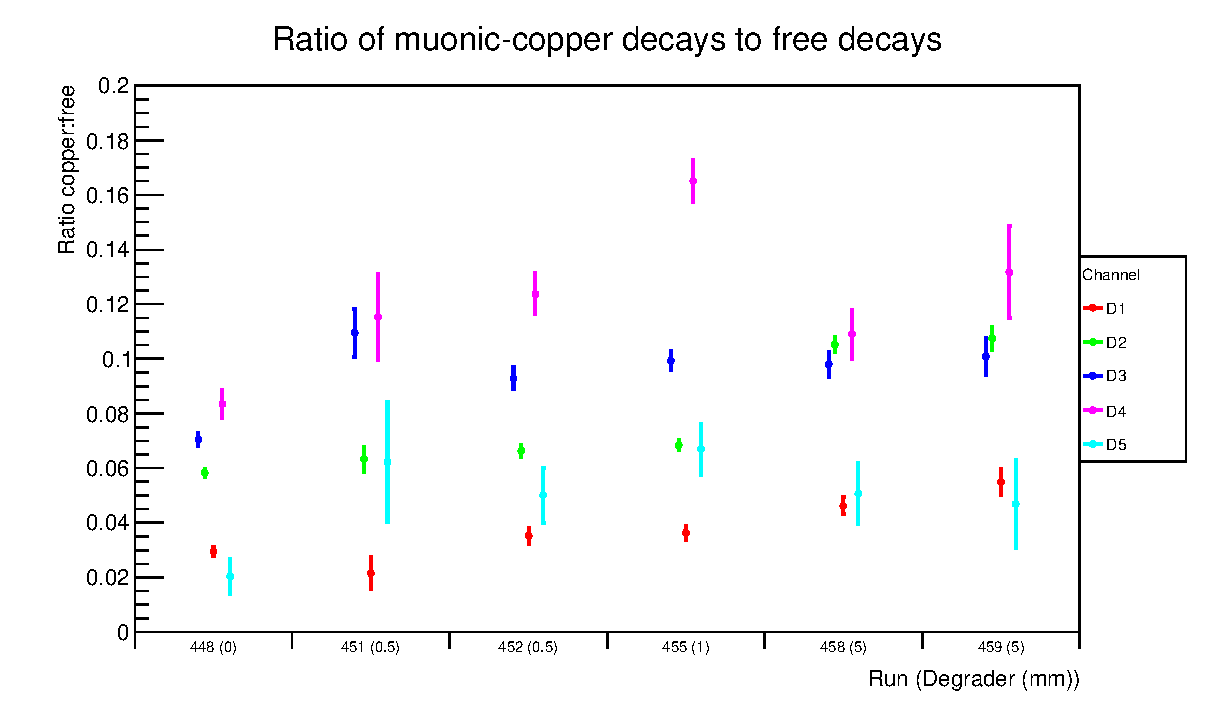
\includegraphics[width=.9\textwidth]{images/plot_generating_scripts/Ratio.eps}
  \caption{Ratio of copper to free decays. The X-axis shows the degrader thickness whilst the colour indicates channel.}
  \label{fig:images_plot_generating_scripts_Ratio}
\end{figure}

\begin{figure}[hptb]
  \centering
    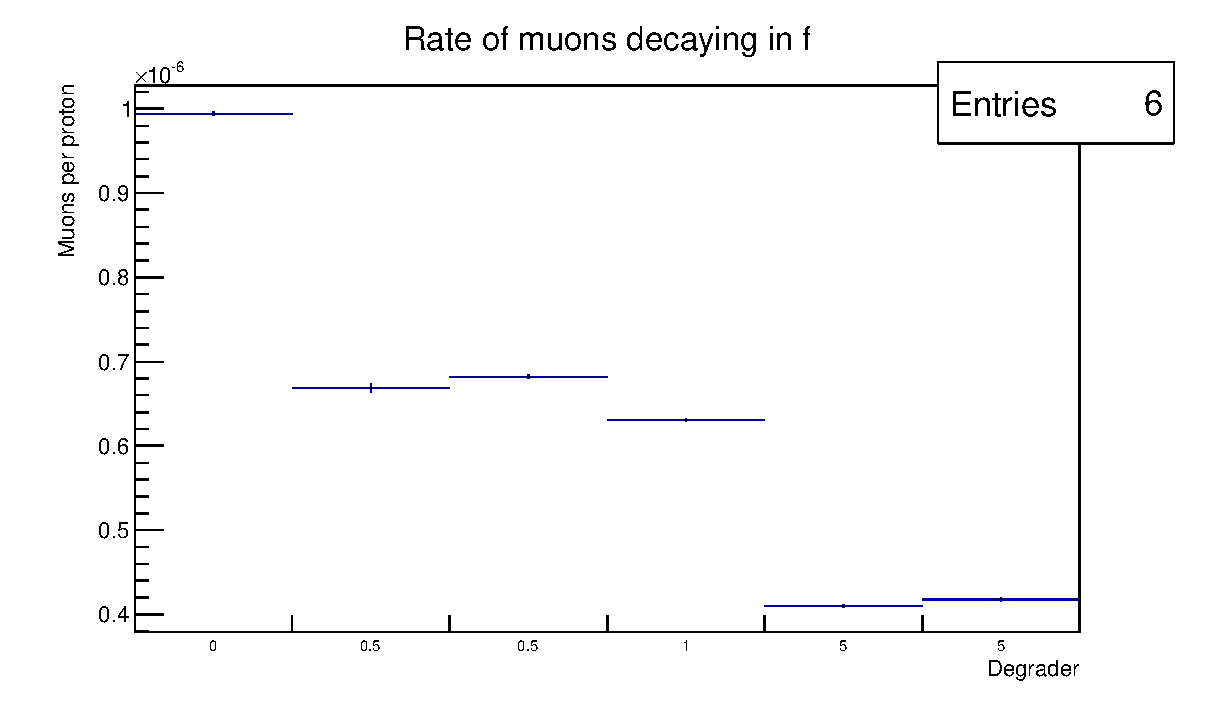
\includegraphics[width=.9\textwidth]{images/momentum_spectrum/run_muon_rate_in_f.eps}
  \caption{Integrated number of free muon decays summed over all channels.}
  \label{fig:images_momentum_spectrum_run_muon_rate_in_f}
\end{figure}

\begin{figure}[hptb]
  \centering
    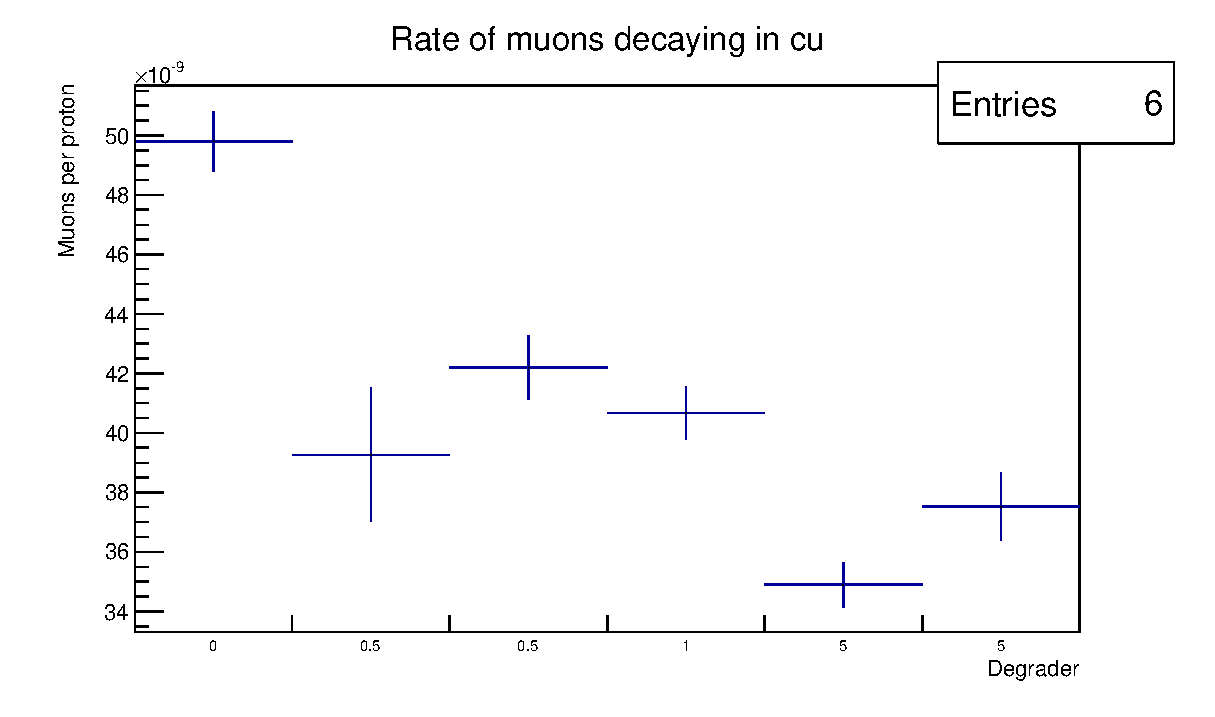
\includegraphics[width=.9\textwidth]{images/momentum_spectrum/run_muon_rate_in_cu.eps}
  \caption{Integrated number of muon decays in copper summed over all channels.}
  \label{fig:images_momentum_spectrum_run_muon_rate_in_cu}
\end{figure}
\clearpage
Once the muon rates (figure~\ref{fig:images_momentum_spectrum_run_muon_rate_in_f}) have been calculated they can be adjusted to account for other affects. This is shown in figure~\ref{fig:images_plot_generating_scripts_adjusted_muon_rates} where additional terms have been incorporated to account for the photon acceptance, the systematic errors due to fitting of curve and the efficiency of the MPPCs. The photon acceptance is taken to be the ratio of muon that decay in a detectable manner to those decay events that produce detected photons. A detectable decay is one where a muon is present in the upstream scintillator and its daughter electron in the downstream scintillator whilst the requirements for detected photons are that the photons must exceed the threshold of that scintillator as well as having an upstream/downstream separation of greater than 50~ns. The efficiency is taken to be twice the product of the average efficiency of one MPPC from section~\ref{sec:detector_efficiency}. The adjusted decay rate, \(R_a\), is then given by:
\begin{align}
    R_a &= \frac{N_{\mu}}{I_p D E \epsilon_{\text{MPPC}}^2 A } \label{equ:adj_rate}
\end{align}
Where the symbols \(I_p\), \(D\) and \(E\) have the same meaning as in equation~\eqref{equ:rate}. Furthermore \(\epsilon_{\text{MPPC}}\) is the average efficiency of an MPPC as determined in section~\ref{sec:detector_efficiency} and \(A\) is the photon acceptance as determined by simulation (see section~\ref{WRITE THIS SECTION ON PHOTON ACCEPTANCE}). 

The same protocol can be applied to the muonic copper decays to get an adjusted rate that is shown in figure~\ref{fig:images_plot_generating_scripts_adjusted_muon_rates_cu} and table~\ref{tab:adjusted_cu_rates}.

\begin{table}
  \begin{center}
  \begin{tabular}{c | c | c | c | c}
    Momentum  & \multirow{2}{*}{Runs}  &  Rate           &  \multicolumn{2}{c}{Error (nA\(^{-1}\))} \\
     (MeV/c)  &                        &  (nA\(^{-1}\))  &     (incl.\ eff.)  &  (excl.\ eff.)      \\
    \hline
    41.0  &       448  &  41,945  &  9,301  &  731  \\
    46.7  &  451, 452  &  28,497  &  6,320  &  507  \\
    50.3  &       455  &  26,604  &  5,900  &  467  \\
    65.7  &  458, 459  &  17,472  &  3,875  &  308  \\
  \end{tabular}
  \end{center}
  \caption{Adjusted rates for freely decaying muons. The error column shows the error without the contribution from the MPPC efficiency and with it, as is clear this is the dominate source.}
  \label{tab:adjusted_free_decay_rates}
\end{table}

\begin{table}
  \begin{center}
  \begin{tabular}{c | c | c | c | c}
    Momentum  & \multirow{2}{*}{Runs}  &  Rate           &  \multicolumn{2}{c}{Error (nA\(^{-1}\))} \\
     (MeV/c)  &                        &  (nA\(^{-1}\))  &     (incl.\ eff.)  &  (excl.\ eff.)      \\
    \hline
    41.0  &       448  &  1580  &  352  &  42  \\
    46.7  &  451, 452  &  1293  &  289  &  45  \\
    50.3  &       455  &  1291  &  288  &  36  \\
    65.7  &  458, 459  &  1149  &  256  &  29  \\
  \end{tabular}
  \end{center}
  \caption{Adjusted rates of muonic copper decay. Errors are split into the dominant portion (due to MPPC efficiency) and other sources.}
  \label{tab:adjusted_cu_rates}
\end{table}

\begin{figure}[hptb] 
  \centering
    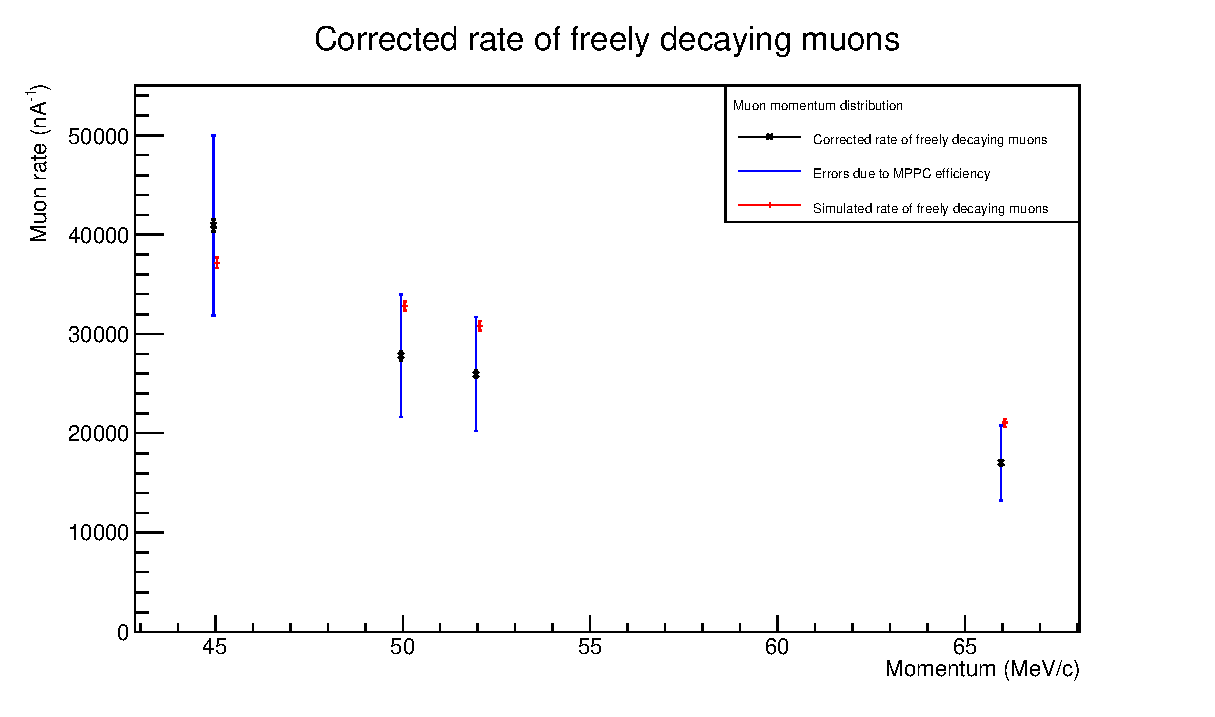
\includegraphics[width=.9\textwidth]{images/plot_generating_scripts/adjusted_muon_rates.eps}
  \caption{Adjusted free muon decay rate and simulated free muon decay rate. The thin error lines for the measured rate indicate the error due to MPPC efficiency whilst the thicker line are due to the remainder of the errors (mainly statistical).}
  \label{fig:images_plot_generating_scripts_adjusted_muon_rates}
\end{figure}

\begin{figure}[hptb]
  \centering
    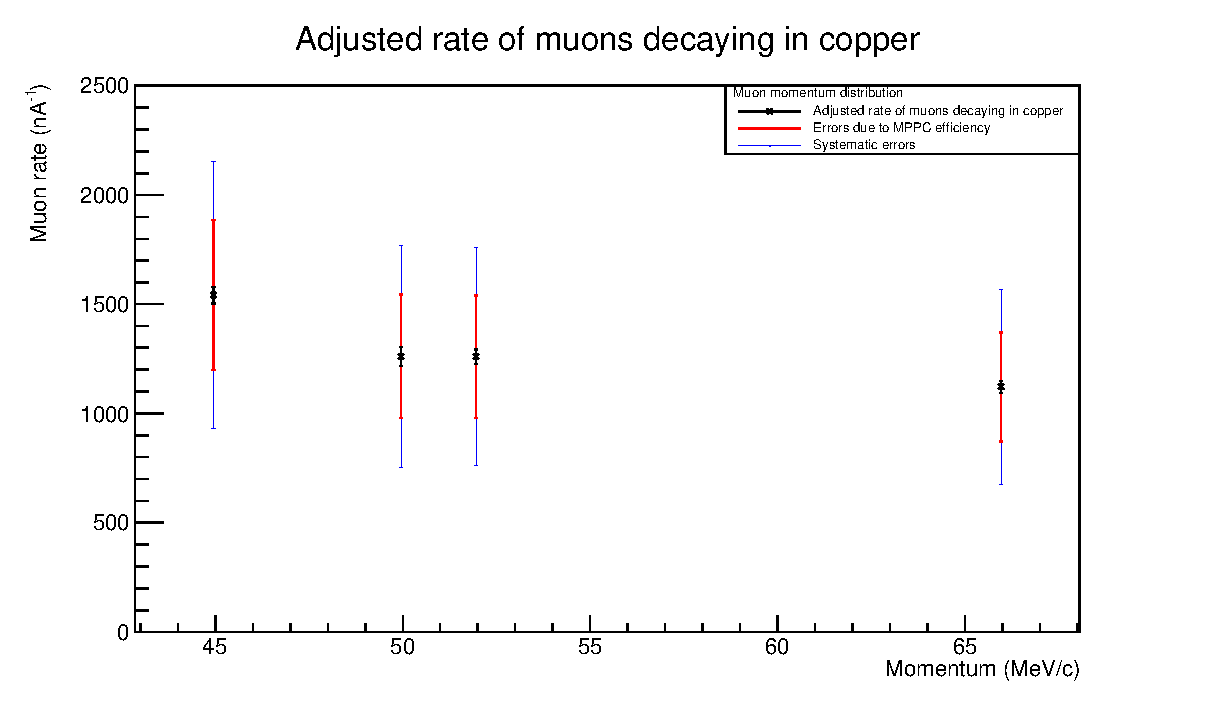
\includegraphics[width=.9\textwidth]{images/plot_generating_scripts/adjusted_muon_rates_cu.eps}
  \caption{Adjusted decay rate of muonic copper. The simulated rates are not shown as the statistics for muonic copper decays were too low to extract reasonable values from. As with the freely decaying muons the thinner error lines are due to the uncertainty on the MPPC efficiency and the thicker lines due to statistics and the other factors.}
  \label{fig:images_plot_generating_scripts_adjusted_muon_rates_cu}
\end{figure}

\subsection{Systematics} % (fold)
\label{sub:systematics}

% subsection systematics (end)
% 
% \label{sec:results}
% % section results (end)
% \section{Analysis} % (fold)
% \label{sec:analysis}



